\documentclass[letterpaper,oneside]{book}
\usepackage[letterpaper,left=1in,right=1in,top=1in,bottom=1in]{geometry}
\usepackage{setspace,epsfig,subfigure,rawfonts,graphicx,graphicx,epsf,psfrag}
\usepackage{amssymb,amsfonts,amsmath,amsthm}
\usepackage[noadjust]{cite}
\usepackage[utf8]{inputenc}
\usepackage{appendix}
\usepackage{array}
\usepackage{eqparbox}
\usepackage{multirow}
\let\counterwithout\relax
\let\counterwithin\relax
\usepackage{chngcntr}
\usepackage{etoolbox}
\usepackage[chapter]{algorithm}
\usepackage{algorithmic}
\usepackage{bm}
\usepackage{titlesec}
\usepackage{lipsum}
\usepackage[nottoc,notlot,notlof]{tocbibind}
\usepackage{physics}
\usepackage[autostyle]{csquotes}
\usepackage{cmbright}
\usepackage[T1]{fontenc}

\renewcommand{\bibname}{References}

\AtBeginEnvironment{subappendices}{%
\chapter*{Appendix}
\addcontentsline{toc}{chapter}{Appendices}
\counterwithin{figure}{chapter}
\counterwithin{table}{chapter}
% \renewcommand{\thefigure}{\arabic{chapter}.\arabic{figure}}
% \renewcommand{\thetable}{\arabic{chapter}.\arabic{table}}
}

\titleformat{\chapter}[display]
{\normalfont\LARGE\bf}
{\chaptertitlename\ \thechapter}{15pt}{}
  
\titlespacing*{\chapter}{0pt}{-20pt}{40pt}

\newcounter{exercisectr}
\newenvironment{exercise}[1][]{%      define a custom environment
  \medskip\noindent%         create a vertical offset to previous material
  \refstepcounter{exercisectr}% increment the environment's counter
  \large{\textbf{Ex. \theexercisectr\ #1}}% or \textbf, \textit, ...
  \newline%
  \setcounter{exerciseSectionctr}{0}
}{\par\medskip}  %          create a vertical offset to following material
\numberwithin{exercisectr}{chapter}

\newcounter{exerciseSectionctr}
\newenvironment{exerciseSection}{
  \medskip\noindent%         create a vertical offset to previous material
  \refstepcounter{exerciseSectionctr}% increment the environment's counter
  \textbf{(\alph{exerciseSectionctr})\ }% or \textbf,.
}

\newtheorem{theorem}{Theorem}
\newtheorem{lemma}{Lemma}
\newtheorem{property}{Property}
\newtheorem{proposition}{Proposition}
\newtheorem{definition}{Definition}
\numberwithin{theorem}{chapter} % important bit
\numberwithin{lemma}{chapter} % important bit
\numberwithin{proposition}{chapter} % important bit

\begin{document}

\doublespacing
\renewcommand{\labelenumi}{(\arabic{enumi})}

\title{
  { A working Solution Manual for: \emph{The Elements of Statistical
  Learning} by Jerome Friedman, Trevor Hastie and Robert Tibshirani}
}

\author{
  Hanchen Wang\\%, hw501@cam.ac.uk\\
  Department of Engineering, University of Cambridge\\
}
\date{\today}
\maketitle

\onehalfspacing
\pagenumbering{roman}
\tableofcontents

%\newpage
\pagenumbering{arabic}
%\newpage
\chapter*{Preface}
\addcontentsline{toc}{chapter}{Preface}

This work is expected to be used as a supplementary material for Weatherwax and
Epstein's solution manual~\cite{weatherwax2013solution}, which I found to be
very helpful when self-studying this popular textbook. The numbering of chapters
and problems are based on the 2nd edition (10th printing with corrections, Jan 2013) available
online~\cite{friedman2009elements}.

The author has just started to solve all the excercises. Even for the solutions
included we expect many mistakes and shortcomings. It would be of great help if
people could suggest possible solutions or help us find and correct the errors
so this solution manual can be continuously improved to benefit more interested
readers. We are also open to all comments and criticisms. The contact
information can be found at the website holding this draft: $https://hansen7.github.io$.


\chapter*{Acknowledgment}
\addcontentsline{toc}{chapter}{Acknowledgment}

\setcounter{chapter}{1}
\chapter{Overview of Supervised Learning}
\label{ch:2} % Chapter 2
\chapter{Linear Methods for Regression}
\label{ch:3} % Chapter 3
\chapter{Linear Methods for Classification}
\label{ch:4} % Chapter 4
\chapter{Basis Expansions and Regularization}
\label{ch:5} % Chapter 5
\chapter{Kernel Smoothing Methods}
\label{ch:6}

\begin{exercise}
  For Gaussian kernel, since $K_{\lambda}(x_0,x_i)$ is differentiable w.r.t.
  $x_0$, we have
  \begin{align}
    \dv{\hat{f}(x_0)}{x_0} &= \frac{\left(\sum_{i=1}^Ny_iK'_{\lambda}(x_0,
    x_i)\right) \left(\sum_{i=1}^NK_{\lambda}(x_0,
    x_i)\right) - \left(\sum_{i=1}^NK'_{\lambda}(x_0,
    x_i)\right)\left(\sum_{i=1}^Ny_iK'_{\lambda}(x_0,
    x_i)y_i\right)} {\left(\sum_{i=1}^NK_{\lambda}(x_0,
    x_i)\right)^2}
  \end{align}
  
  Since Epanechnikov kernel is not differentiable, the corresponding
  Nadaraya-Watson kernel smooth function is not differentiable, either.
\end{exercise}

\begin{exercise}
  Denote $\mathbf{l}(x_0) = [l_1(x_0),\ldots,l_N(x_0)]^T$ as a $N$-by-1 vector.
  From Eq. (6.8) we can see that
  \begin{align}
    \mathbf{l}^T(x_0) &= \mathbf{b}(x_0)^T
    \left(\mathbf{B}^T\mathbf{W}(x_0)\mathbf{B}\right)^{-1}
    \mathbf{B}^T\mathbf{W}(x_0)
  \end{align}
  therefore
  \begin{align}
    \mathbf{l}^T(x_0)\mathbf{B} &= \left[\sum_{i=1}^Nl_i(x_0),\ldots,
    \sum_{i=1}^Nl_i(x_0)x_i^{k}\right] \notag\\
    &= \mathbf{b}^T(x_0) = [1, \ldots, x_0^{k}]
  \end{align}
  which suggests that 
  \begin{align}
    \sum_{i=1}^Nl_i(x_0)x_i^{j} = x_0^j,\,j=0.\ldots,k
  \end{align}
  \begin{itemize}
    \item When $j=0$, we have $\sum_{i=1}^Nl_i(x_0) = 1$.
    \item When $j>0$, since 
    \begin{align}
      \sum_{i=1}^Nl_i(x_0)x_i^{j} &= x_0^j  = x_0^l\cdot x_0^{j-l} =
      \sum_{i=1}^Nl_i(x_0)x_i^{l}x_0^{j-l}
    \end{align}
    for any $0\leq l\leq j$, it is easy to verify that 
    \begin{align}
      \sum_{i=1}^Nl_i(x_0)(x_i - x_0)^j = 0.
    \end{align}
    which suggests that the bias is 0 to order $k$ according to Eq. (6.10). 
  \end{itemize}
  
\end{exercise}

\begin{exercise}
  ???
\end{exercise}

\begin{exercise}
  The Mahalanobis choice of $\mathbf{A} = \mathbf{\Sigma}^{-1}$ has the effect
  of ``eqaulizaing'' the distance measure in each dimension according to how the
  data vary over that dimension, while $\mathbf{A} = \mathbf{I}$ results in the
  Euclidean distance which ignores the distribution of the data $\mathbf{X}$.
  
  A kernel that downweightshigh-frequency components in the
  distance metric can be constructed as $\mathbf{A} = \mathbf{F}^T\mathbf{F}$,
  where the rows of $\mathbf{F}$ are the cyclic-shifted version of a low-pass
  filter. In this way, $\mathbf{Fx}$ represents the circular convolution of the
  filter and the samples $\mathbf{x}$ which rejects high frequency components.
  To ignore high-frequency components completely, we can simply define
  $\mathbf{F}$ as a all-1 matrix.
\end{exercise}

\begin{exercise}
  Denote the binary response indicator vector for the $i$-th record as
  $\mathbf{y}_i$, such that $y_{ij}=1$ if $g_i=j$ and otherwise $y_{ij}=0$,
  $j=1,\ldots,J$. Then the local log-likelihood can be rewritten as
  \begin{align}
    l(\bm{\beta}) &= \sum_{i=1}^N K_{\lambda}(x_0, x_i)
    \left[\sum_{j=1}^{J-1}y_{ij}\log\mbox{Pr}(G=j|X=x_i)  +
    \left(1-\sum_{j=1}^{J-1}y_{ij}\right) \log\mbox{Pr}(G=J|X=x_i) \right]
    \notag\\ &=
    \sum_{i=1}^N K_{\lambda}(x_0, x_i)
    \left[\sum_{j=1}^{J-1}y_{ij}\beta_{j0}(x_0)
    -\log\left(1+\sum_{j=1}^{J-1} \exp(\beta_{j0}(x_0)) \right) \right]
  \end{align} 
  To maximize the log-likelihood, setting the derivative w.r.t $\beta_{j0}$ to 0
  results in
  \begin{align}
    \pdv{l(\bm{\beta})}{\beta_{j0}(x_0)} = \sum_{i=1}^N K_{\lambda}(x_0,
    x_i)\left(y_{ij} - p_j\right) = 0
  \end{align}
  where
  \begin{align}
    p_j &= \frac{\exp(\beta_{j0}(x_0))}{1 + \sum_{k=1}^{J-1}
    \exp(\beta_{k0}(x_0))}
  \end{align}
  therefore $\beta_{j0}, j=1,\ldots,J-1$ should be selected such that
  \begin{align}
    p_j &= \frac{\sum_{i=1}^N K_{\lambda}(x_0,x_i)y_{ij}} {\sum_{i=1}^N
    K_{\lambda}}
  \end{align}
  which amounts to smoothing the binary response indicators for each class
  separately using a Nadaraya–Watson kernel smoother with kernel weights
  $K_{\lambda}(x_0,x_i)$.
\end{exercise}

\begin{exercise}
  Divide the set of monomials into $Z$ and $X$. Define kernel on $Z$ and use
  $X$ as predictors. Given a new input $[\mathbf{z}_0, \mathbf{x}_0]$, fit local
  regression model as
  \begin{align}
    \min_{\alpha(\mathbf{z}_0),
    \bm{\beta}(\mathbf{z}_0)}\sum_{i=1}^NK_{\lambda}(\mathbf{z}_0,\mathbf{z}_i)
    (y_i-\alpha(\mathbf{z}_0) - \mathbf{x}_i^T\bm{\beta}(\mathbf{z}_0) )
  \end{align}
\end{exercise}

\begin{exercise}
  \begin{align}
    \frac{1}{N} \sum_{k=1}^N \sum_{i\not=k}
    K_{\lambda}(\mathbf{x}_i,\mathbf{x}_k) (y_i - \alpha_k -
    \mathbf{x}_i^T\bm{\beta}_k)
  \end{align}
\end{exercise}

\begin{exercise}
  The Parzen density estimate for $X, Y$ jointly and $X$ alone are
  \begin{subequations}
    \begin{align}
      \hat{f}_{X,Y}(x,y) & = \frac{1}{N}\sum_{i=1}^N
      \phi_{\lambda}(x-x_i)\phi_{\lambda}(y-y_i) \\
      \hat{f}_{X}(x) & = \frac{1}{N}\sum_{i=1}^N
      \phi_{\lambda}(x-x_i)
    \end{align}
  \end{subequations}
  respectively, therefore
  \begin{align}
    \mathbb{E}[Y|X] &= \int y \frac{\hat{f}_{X,Y}(x,y)}{\hat{f}_{X}(x)}dy
    \notag\\ &=
    \frac{\sum_{i=1}^N \phi_{\lambda}(x-x_i) \int y\phi_{\lambda}(y-y_i)dy}
    {\sum_{i=1}^N\phi_{\lambda}(x-x_i)}
  \end{align}
  which is a Nadaraya-Watson estimator. 
  
  For classification we adopt the
  product kernel $\phi_{\lambda}(X)\delta(g)$, where $\delta(\cdot)$ is the
  Kronecker delta function. As a result, the Parzen density estimate for $X, G$
  jointly is
  \begin{align}
    \hat{f}_{X,G}(x,g) & = \frac{1}{N}\sum_{i=1}^N
    \phi_{\lambda}(x-x_i)\delta(g=g_i)
  \end{align}
  therefore the probability estimation is
  \begin{align}
    \mbox{Pr}(G=g|X=x) = \frac{\hat{f}_{X,G}(x,g)} {\hat{f}_{X}(x)} =
    \frac{\sum_{g_i=g}\phi_{\lambda}(x-x_i)} {\sum_{i=1}^N\phi_{\lambda}(x-x_i)}
  \end{align}
\end{exercise}

\begin{exercise}
  Naive bayesian model makes a stronger assumption that given a class $G = j$
  the features $X_k$ are independent as in Eq. (6.27), which leads to the
  additive form of the log-likelihood function in Eq. (6.27)  On the contrary
  the GAM model directly assumes a additive form of the log-likelihood function
  (Eq. (9.8)) and no specific form of the distribution function is assumed.
  
  Naive bayesian model enables the estimation of the 1-D density function of the
  features conditioned on class $f_{jk}$ , while in the GAM model the additive
  components $f_1,\ldots, f_p$ are estimated by a iterative backfitting
  algorithm.
\end{exercise}

\begin{exercise}
  \begin{align}
    \mathbb{E}\left[\mbox{ASR}(\lambda)\right] & = \frac{1}{N}
    \mathbb{E}\left[ \|\mathbf{y} - \mathbf{S}_{\lambda}\mathbf{y}\|^2\right]
    \notag\\
    &= \frac{1}{N}\mathbb{E}\left[\|(\mathbf{f} + \bm{\epsilon}) -
    \mathbf{S}_{\lambda}(\mathbf{f} + \bm{\epsilon})\|^2 \right] \notag\\
    &= \frac{1}{N} \|\mathbf{f} - \mathbf{S}_{\lambda}\mathbf{f}\|^2 +
    \frac{1}{N} \mathbb{E}\left[\|\bm{\epsilon} -
    \mathbf{S}_{\lambda}\bm{\epsilon})\|^2 \right] \notag \\
    &= \frac{1}{N} \|\mathbf{f} - \mathbf{S}_{\lambda}\mathbf{f}\|^2 +
    \frac{\left[N - 2\mbox{tr}(\mathbf{S}_{\lambda}) +
    \mbox{tr}(\mathbf{S}_{\lambda}\mathbf{S}_{\lambda}^T)\right]\sigma^2}{N}
  \end{align}
  \begin{align}
    \mbox{PE}(\lambda) & = \frac{1}{N}\mathbb{E}\left[\|\mathbf{y}^* -  
    \mathbf{S}_{\lambda}\mathbf{y}\|^2 \right] \notag\\
    &= \frac{1}{N}\mathbb{E}\left[\|(\mathbf{f} + \bm{\epsilon}^*) -
    \mathbf{S}_{\lambda}(\mathbf{f} + \bm{\epsilon})\|^2 \right] \notag\\
    &= \frac{1}{N} \|\mathbf{f} - \mathbf{S}_{\lambda}\mathbf{f}\|^2 +
    \frac{1}{N} \mathbb{E}\left[\|\bm{\epsilon}^* -
    \mathbf{S}_{\lambda}\bm{\epsilon})\|^2 \right] \notag \\
    &= \frac{1}{N} \|\mathbf{f} - \mathbf{S}_{\lambda}\mathbf{f}\|^2 +
    \frac{\left[N +
    \mbox{tr}(\mathbf{S}_{\lambda}\mathbf{S}_{\lambda}^T)\right]\sigma^2}{N}
  \end{align}
  therefore
  \begin{align}
    \mbox{PE}(\lambda) & =  \mathbb{E}\left[\mbox{ASR}(\lambda)\right] +
    \frac{2\mbox{tr}(\mathbf{S}_{\lambda})\sigma^2}{N} =
    \mathbb{E}\left[ C_{\lambda}\right]
  \end{align}
\end{exercise}

\begin{exercise}
  The likelihood is maximized to $+\infty$ by setting any $\bm{\mu}_m$ to a
  record $\mathbf{x}_i$ and setting $\mathbf{\Sigma} = \mathbf{0}$.
\end{exercise}

\begin{exercise}[(Program)]
\end{exercise}
 % Chapter 6
\chapter{Model Assessment and Selection}
\label{ch:7}

\begin{exercise}
  \begin{align}
    \mathbb{E}_{\mathbf{y}}\left[\mbox{Err}_{\mbox{in}}\right] &= \frac{1}{N}
    \mathbb{E}_{\mathbf{y},
    \mathbf{y}^0}\left[\|\mathbf{y}^0 - \hat{f}(\mathbf{x})\|^2|\mathcal{T} \right] \notag \\
    &= \frac{1}{N}
    \mathbb{E}_{\mathbf{y},\mathbf{y}^0}\left[
    \|\mathbf{y}^0 -
    \mathbf{X}(\mathbf{X}^T\mathbf{X})^{-1}\mathbf{X}^T\mathbf{y}\|^2|\mathcal{T}
     \right] \notag \\
    &= \frac{1}{N}
    \mathbb{E}_{\mathbf{y},\mathbf{y}^0}\left[\|(\mathbf{y}^0 -
    \mathbf{X}(\mathbf{X}^T\mathbf{X})^{-1}\mathbf{X}^T\mathbf{y}^0) + 
     \mathbf{X}(\mathbf{X}^T\mathbf{X})^{-1}\mathbf{X}^T(\mathbf{y}^0 -
     \mathbf{y})\|^2|\mathcal{T}
    \right] \notag \\
    &= \frac{1}{N} \mathbb{E}_{\mathbf{y}^0} \left[\|(\mathbf{y}^0 -
    \mathbf{X}(\mathbf{X}^T\mathbf{X})^{-1}\mathbf{X}^T\mathbf{y}^0)\|^2\right]
    +
    \frac{1}{N}
    \mathbb{E}_{\bm{\epsilon}, \bm{\epsilon}^0}\left[
    \|\mathbf{X}(\mathbf{X}^T\mathbf{X})^{-1}\mathbf{X}^T(\bm{\epsilon}^0 -
    \bm{\epsilon})\|^2 \right] \notag\\
    &= \mathbb{E}_{\mathbf{y}}(\overline{\mbox{err}}) +
    \frac{2\sigma_{\epsilon}^2}{N}\mbox{tr}\left(\mathbf{X}(\mathbf{X}^T\mathbf{X})^{-1}\mathbf{X}^T
    \right) \notag\\
    &= \mathbb{E}_{\mathbf{y}}(\overline{\mbox{err}}) +
    \frac{2d}{N}\sigma_{\epsilon}^2
  \end{align}
\end{exercise}

\begin{exercise}
  \begin{align}
    \mbox{Err}(x_0) &= \mbox{Pr}(Y\not= \hat{G}(x_0)|X=x_0) \notag\\
    &= \mbox{Pr}(Y\not= G(x_0)|X=x_0)\left[
    \mbox{Pr}(G(x_0)=\hat{G}(x_0)|X=x_0) +
    \mbox{Pr}(G(x_0)\not=\hat{G}(x_0)|X=x_0)\right] \notag\\
    &+ \left[\mbox{Pr}(Y=G(x_0)|X=x_0) - \mbox{Pr}(Y\not=G(x_0)|X=x_0)\right]
    \mbox{Pr}(G(x_0)\not=\hat{G}(x_0)|X=x_0) \notag\\
    &= \mbox{Err}_{\mbox{B}}(x_0) + \left[\mbox{Pr}(Y=G(x_0)|X=x_0) -
    \mbox{Pr}(Y\not=G(x_0)|X=x_0)\right]\mbox{Pr}(G(x_0)\not=\hat{G}(x_0)|X=x_0)
    \notag\\
    &= \mbox{Err}_{\mbox{B}}(x_0)  +
    |1-2f(x_0)|\mbox{Pr}(G(x_0)\not=\hat{G}(x_0)|X=x_0)
  \end{align}
  
  \begin{itemize}
    \item If $f(x_0)\geq 1/2$ therefore $G(x_0)=1$, we have
    \begin{align}
      \mbox{Pr}(G(x_0)\not=\hat{G}(x_0)|X=x_0) =
      \mbox{Pr}(\hat{f}(x_0)<1/2) \approx
      \Phi\left(\frac{-\mathbb{E}\left[\hat{f}(x_0)\right]+1/2 }
      {\sqrt{\mbox{var}(\hat{f}(x_0))}}\right)
    \end{align}
    \item Otherwise $f(x_0)< 1/2$ thus $G(x_0)=0$, we have
    \begin{align}
      \mbox{Pr}(G(x_0)\not=\hat{G}(x_0)|X=x_0) =
      \mbox{Pr}(\hat{f}(x_0)\geq1/2) \approx
      \Phi\left(\frac{\mathbb{E}\left[\hat{f}(x_0)\right]-1/2}
      {\sqrt{\mbox{var}(\hat{f}(x_0))}}\right)
    \end{align}
  \end{itemize}
  Consequently, Eq. (7.63) is proved.
\end{exercise}

\begin{exercise}
  \begin{exerciseSection}
    Denote $\mathbf{x}_i$ as the column vector representing the $i$-th record,
    i.e. the transpose of the $i$-th row of $\mathbf{X}$.
    \begin{align}
      y_i-\hat{f}^{-i}(\mathbf{x}_i) =
      y_i-\mathbf{x}_i^T(\mathbf{X}_{-i}^T\mathbf{X}_{-i})^{-1}
      \mathbf{X}_{-i}^T\mathbf{y}_{-i}
    \end{align}
    where
    \begin{subequations}
      \begin{align}
        (\mathbf{X}_{-i}^T\mathbf{X}_{-i})^{-1} &= \left(\mathbf{X}^T\mathbf{X} -
        \mathbf{x}_i\mathbf{x}_i^T \right)^{-1} \notag\\
        &= \left(\mathbf{X}^T\mathbf{X}\right)^{-1} - 
        \left(\mathbf{X}^T\mathbf{X}\right)^{-1} \mathbf{x}_i\left(-1 +
        \mathbf{x}_i^T(\mathbf{X}^T\mathbf{X})^{-1}\mathbf{x}_i\right)^{-1}\mathbf{x}_i^T
        \left(\mathbf{X}^T\mathbf{X}\right)^{-1} \notag\\
        &= \left(\mathbf{X}^T\mathbf{X}\right)^{-1} + \frac{1}{1-S_{ii}}
        \left(\mathbf{X}^T\mathbf{X}\right)^{-1} \mathbf{x}_i\mathbf{x}_i^T
        \left(\mathbf{X}^T\mathbf{X}\right)^{-1} \\
        \mathbf{X}_{-i}^T\mathbf{y}_{-i} &= \mathbf{X}^T\mathbf{y}
        -\mathbf{x}_iy_i
      \end{align}
    \end{subequations}
    therefore
    \begin{align}
      y_i-\hat{f}^{-i}(\mathbf{x}_i) &= y_i -
      \left[\mathbf{x}_i^T\left(\mathbf{X}^T\mathbf{X}\right)^{-1}\mathbf{X}^T\mathbf{y}
      + \frac{1}{1-S_{ii}} \mathbf{x}_i^T
      \left(\mathbf{X}^T\mathbf{X}\right)^{-1} \mathbf{x}_i\mathbf{x}_i^T
      \left(\mathbf{X}^T\mathbf{X}\right)^{-1} \mathbf{X}^T\mathbf{y}\right.
      \notag\\
      & -  
      \left. \mathbf{x}_i^T\left(\mathbf{X}^T\mathbf{X}\right)^{-1}
      \mathbf{x}_iy_i -
      \frac{1}{1-S_{ii}} \mathbf{x}_i^T \left(\mathbf{X}^T\mathbf{X}\right)^{-1}
      \mathbf{x}_i\mathbf{x}_i^T \left(\mathbf{X}^T\mathbf{X}\right)^{-1}
      \mathbf{x}_iy_i\right] \notag\\
      &= y_i - \left[\hat{f}(\mathbf{x}_i) +
      \frac{S_{ii}}{1-S_{ii}}\hat{f}(\mathbf{x}_i) - S_{ii}y_i -
      \frac{S_{ii}^2}{1-S_{ii}}y_i \right]\notag\\
      &= \frac{1}{1-S_{ii}}\left(y_i - \hat{f}(\mathbf{x}_i) \right)
    \end{align}
  \end{exerciseSection}
  \begin{exerciseSection}
    Since $\mathbf{S} = \mathbf{UU}^T$, where $\mathbf{X} = \mathbf{UDV}^T$ is
    the SVD of $\mathbf{X}$, $0\leq S_{ii}\leq 1$, thus
    \begin{align}
      \left|y_i-\hat{f}^{-i}(\mathbf{x}_i)\right| \geq
      \left|y_i-\hat{f}(\mathbf{x}_i)\right|
    \end{align}
  \end{exerciseSection}
  \begin{exerciseSection}
    ???
  \end{exerciseSection}
\end{exercise}

\begin{exercise}
  Denote $\hat{f}(\mathbf{x}_i) = \hat{y}_i$ (which of course also depends on
  $\mathbf{X}$, $\mathbf{y}$), then
  \begin{align}
    \mathbb{E}_{\mathbf{y}}[\mbox{Err}_{\mbox{in}}] -
    \mathbb{E}_{\mathbf{y}}[\overline{\mbox{err}}] & =
    \frac{1}{N}\mathbb{E}_{\mathbf{y}, \mathbf{y}^0} \left[\sum_{i=1}^N
    \|y_i^0 - \hat{y}_i\|^2 \right] - \frac{1}{N} \mathbb{E}_{\mathbf{y},
    \mathbf{y}^0} \left[\sum_{i=1}^N \|y_i - \hat{y}_i\|^2 \right] \notag\\
    &= \frac{2}{N}\sum_{i=1}^N \mathbb{E}_{\mathbf{y}}\left[y_i\hat{y}_i \right]
    - \mathbb{E}_{\mathbf{y},\mathbf{y}^0}\left[y_i^0\hat{y}_i \right] \notag\\
    &= \frac{2}{N}\sum_{i=1}^N \mathbb{E}_{\mathbf{y}}\left[y_i\hat{y}_i \right]
    - \mathbb{E}_{\mathbf{y}}\left[y_i\right]
    \mathbb{E}_{\mathbf{y}}\left[\hat{y}_i \right] \notag\\
    &= \frac{2}{N}\sum_{i=1}^N\mbox{cov}(y_i, \hat{y}_i)
  \end{align}
\end{exercise}

\begin{exercise}
  \begin{align}
    \sum_{i=1}^N \mbox{cov}(y_i, \hat{y}_i) &= \mbox{tr} \left(\mathbb{E}\left[
    (\mathbf{y} - \bar{\mathbf{y}})(\mathbf{S}(\mathbf{y} -
    \bar{\mathbf{y}}))^T\right] \right) \notag\\
    &= \mbox{tr}\left(\mathbb{E}\left[(\mathbf{y} - \bar{\mathbf{y}})(\mathbf{y}
    - \bar{\mathbf{y}})^T \right]\mathbf{S} \right) \notag\\
    &= \mbox{tr}(\mathbf{S})\sigma_{\epsilon}^2
  \end{align}
\end{exercise}

\begin{exercise}
  For $k$-nearest-neighbor regression, $\mathbf{S}$ equals to $1/k$ times a
  $N$-by-$N$ binary matrix which
  \begin{itemize}
    \item Each row has exactly $k$ 1s and $N-k$ 0s.
    \item The diagonal entries are all 1s.
  \end{itemize}
  Therefore $\mbox{tr}(\mathbf{S}) = N/k$.
\end{exercise}

\begin{exercise}
  \begin{align}
    \mbox{GCV} &= \frac{1}{N(1-d/N)^2}\sum_{i=1}^N\left(y_i -
    \hat{f}(\mathbf{x}_i)\right)^2 \notag\\
    &\approx \frac{1}{N}\left(1 + \frac{2d}{N} \right) \sum_{i=1}^N\left(y_i -
    \hat{f}(\mathbf{x}_i)\right)^2  \notag\\
    &= \overline{\mbox{err}} + \frac{2d}{N}\hat{\sigma}_{\epsilon}^2 \notag\\
    &= C_p
  \end{align}
\end{exercise}

\begin{exercise}
  $\alpha$ can be constructed as
  \begin{align}
    \alpha = \frac{\pi}{2}\left(10^{l+1} + \sum_{i=1}^ld_i10^i\right)
  \end{align}
  where $d_i = 1$ if the $i$-th point is assigned label 0 and $d_i =3$
  otherwise. Apparenty, $\sin(\alpha z^i) <0 $ if $d_i = 1$ and $\sin(\alpha
  z^i) >0 $ otherwise, thus $sin(\alpha x)$ shatters $z^1,\ldots,z^l$.
\end{exercise}

\begin{exercise}[(Program)]
\end{exercise}

\begin{exercise}
  No, this is not the right way to do CV. One should select a different
  predictor individually for each validation set and then carries out the CV.
\end{exercise} % Chapter 7
\chapter{Model Inference and Averaging}
\label{ch:8}

\begin{exercise}
  Since $\log(\cdot)$ is a concave function, we have
  \begin{align}
    \mathbb{E}_q\left[\log(r(Y) / q(Y)) \right] &
    \leq\log\left(\mathbb{E}_q\left[(r(Y) / q(Y)\right]\right) \notag\\
    & = \log\left(\int_yr(y)dy \right) \notag \\
    &= 0
  \end{align}
  where equality holds iff $r(Y) = q(Y)$. Consequently
  \begin{align}
    R(\theta',\theta) - R(\theta, \theta) & =
    \mathbb{E}_{\mathbf{T|\mathbf{Z},\theta}}
    \left[\log\mbox{Pr}(\mathbf{Z}^m|\mathbf{Z},\theta') -
    \log\mbox{Pr}(\mathbf{Z}^m|\mathbf{Z},\theta)\right] \notag\\
    &= \mathbb{E}_{\mathbf{T|\mathbf{Z},\theta}}
    \left[\log\frac{\mbox{Pr}(\mathbf{Z}^m|\mathbf{Z},\theta')}
    {\mbox{Pr}(\mathbf{Z}^m|\mathbf{Z},\theta)} \right] \notag\\
    \leq 0
  \end{align}
  where equality holds when $\theta=\theta'$.
\end{exercise}

\begin{exercise}
  \begin{align}
    F(\theta',\tilde{P}) &= \mathbb{E}_{\tilde{P}}
    \left[l_0(\theta',\mathbf{T})\right] -
    \mathbb{E}_{\tilde{P}}\left[\log\tilde{P}(\mathbf{Z}^m)) \right] \notag\\
    &= \log P(\mathbf{Z}|\theta') +
    \mathbb{E}_{\tilde{P}}\left[\frac{P(\mathbf{Z}^m|\mathbf{Z},\theta')}
    {\tilde{P}(\mathbf{Z}^m)} \right] \notag\\
    &\leq \log P(\mathbf{Z}|\theta')
  \end{align}
  where equality holds iff
  $\tilde{P}(\mathbf{Z}^m)=P(\mathbf{Z}^m|\mathbf{Z},\theta')$.
\end{exercise}

\begin{exercise}
  \begin{align}
    \widehat{\mbox{Pr}}_{U_k}(u) &= \int\mbox{Pr}\left(u|u_l,
    l\not=k\right) \mbox{Pr}\left(u_l\right)du_l \notag\\
    &\approx\sum_{t=m}^M \mbox{Pr}\left(u|u_l,
    l\not=k\right) \frac{\mbox{count}(U_l^{(t)} = u_l)}{M-m+1} \notag\\
    &= \frac{1}{M-m+1} \sum_{t=m}^M \mbox{Pr}\left(u|U_l^{(t)}, l\not=k\right)
  \end{align}
\end{exercise}

\begin{exercise}
  Since
  \begin{align}
    \hat{f}^*(x) &= \hat{\mu}^*(x) \notag\\
    &= \mathbf{h}(x)^T(\mathbf{H}^T\mathbf{H})^{-1}\mathbf{H}^T
    \left(\mathbf{H}(\mathbf{H}^T\mathbf{H})^{-1}\mathbf{H}^T\mathbf{y} +
    \bm{\epsilon}^* \right) \notag\\
    & \sim \mathcal{N}(\hat{\mu}(x),
    \mathbf{h}(x)^T(\mathbf{H}^T\mathbf{H})^{-1}\mathbf{h}(x)\hat{\sigma}^2)
  \end{align}
  therefore
  \begin{align}
    \hat{f}_{\mbox{bag}}(x) &= \frac{1}{B}\sum_{b=1}^B
    \hat{f}_b^*(x) \sim \mathcal{N}(\hat{\mu}(x),
    \frac{1}{B}
    \mathbf{h}(x)^T(\mathbf{H}^T\mathbf{H})^{-1}\mathbf{h}(x)\hat{\sigma}^2)
  \end{align}
  as different bags are independent. Consequently, as
  $B\rightarrow\infty$, $\hat{f}_{\mbox{bag}}(x) \rightarrow
  \hat{f}(x) = \hat{\mu}(x)$.
\end{exercise}

\begin{exercise}[(Wrong problem from Chapter 10?)]
\end{exercise}

\begin{exercise}[(Program)]
\end{exercise}

\begin{exercise}
  ???
\end{exercise} % Chapter 8
\chapter{Additive Models, Trees, and Related Methods}
\label{ch:9}

\begin{exercise}
  To show that $\mathbf{Sy} = \hat{\mathbf{y}} + \mathbf{Sr} $, it is sufficient
  to show that $\mathbf{S}^2=\mathbf{S}$. For linear regression,
  \begin{align}
    \mathbf{S}^2=[\mathbf{H}(\mathbf{H}^T\mathbf{H})^{-1}\mathbf{H}^T]
    [\mathbf{H}(\mathbf{H}^T\mathbf{H})^{-1}\mathbf{H}^T] 
    =\mathbf{H}(\mathbf{H}^T\mathbf{H})^{-1}\mathbf{H}^T = \mathbf{S}
  \end{align}
  
  For local linear regression, we have
  \begin{align}
    \mathbf{S}^2 & =
    [\mathbf{B}(\mathbf{B}^T\mathbf{W}\mathbf{B})^{-1}\mathbf{B}^T\mathbf{W}] 
    [\mathbf{B}(\mathbf{B}^T\mathbf{W}\mathbf{B})^{-1}\mathbf{B}^T\mathbf{W}]
    \notag\\ &=
    \mathbf{B}(\mathbf{B}^T\mathbf{W}\mathbf{B})^{-1}\mathbf{B}^T\mathbf{W}
    \notag \\ &=
    \mathbf{S} 
  \end{align}
\end{exercise}

\begin{exercise}
  \begin{exerciseSection}
    The $j$-th row-block of Eq. (9.33) corresponds to the following equation:
    \begin{align}
      \mathbf{f}_j + \mathbf{S}_j\sum_{k\not=j}\mathbf{f}_k =  \mathbf{S}_j
      \mathbf{y}
    \end{align}
    for $j=1,\ldots,p$. The solution to $\mathbf{f}_j$ from this equation alone
    is
    \begin{align}
      \mathbf{f}_j\leftarrow \mathbf{S}_j\left[\mathbf{y} -
      \sum_{k\not=j}\mathbf{f}_k\right]
    \end{align}
  \end{exerciseSection}
  
  \begin{exerciseSection}
    Denote the eigen decomposition of $\mathbf{S}_1$ and $\mathbf{S}_1$ as
    $\mathbf{S}_1 = \mathbf{U}_1\mathbf{D}_1\mathbf{U}_1^T$ and $\mathbf{S}_2 =
    \mathbf{U}_2\mathbf{D}_2\mathbf{U}_2^T$.
    
    Let $\tilde{\mathbf{f}}_1 = \mathbf{U}_1^T\mathbf{f}_1$, $\tilde{\mathbf{f}}_2 =
    \mathbf{U}_2^T\mathbf{f}_2$ and $\tilde{\mathbf{y}}_1 =
    \mathbf{D}_1\mathbf{U}_1^T\mathbf{y}$, $\tilde{\mathbf{y}}_2 =
    \mathbf{D}_2\mathbf{U}_2^T\mathbf{y}$. As a result, the 1-step update can be
    written as
    \begin{subequations}
      \begin{align}
        &\mathbf{f}_1 \leftarrow \mathbf{S}_1(\mathbf{y}-\mathbf{f}_2)
        \Longrightarrow  \tilde{\mathbf{f}}_1 \leftarrow
        \tilde{\mathbf{y}}_1- \mathbf{D}_1\tilde{\mathbf{f}}_2\\
        &\mathbf{f}_2 \leftarrow \mathbf{S}_2(\mathbf{y}-\mathbf{f}_1)
        \Longrightarrow  \tilde{\mathbf{f}}_2 \leftarrow
        \tilde{\mathbf{y}}_2- \mathbf{D}_2\tilde{\mathbf{f}}_1
      \end{align}
    \end{subequations}
    thus the 2-step update can be written as
    \begin{subequations}
      \begin{align}
        & \tilde{\mathbf{f}}_1 \leftarrow
        (\tilde{\mathbf{y}}_1-
        \mathbf{D}_1\tilde{\mathbf{y}}_2) + \mathbf{D}\tilde{\mathbf{f}}_1\\
        & \tilde{\mathbf{f}}_2 \leftarrow
        (\tilde{\mathbf{y}}_2-
        \mathbf{D}_2\tilde{\mathbf{y}}_1) + \mathbf{D}\tilde{\mathbf{f}}_2
      \end{align}
    \end{subequations} 
    where $\mathbf{D} = \mathbf{D}_1\mathbf{D}_2 = \mathbf{D}_2\mathbf{D}_1$ is
    a diagonal matrix with entries in $[0, 1)$. Consequently, the iterative
    update converges on
    \begin{subequations}
      \begin{align}
        & \tilde{\mathbf{f}}_1 \rightarrow \mathbf{D}_S (\tilde{\mathbf{y}}_1-
        \mathbf{D}_1\tilde{\mathbf{y}}_2)\\
        & \tilde{\mathbf{f}}_2 \rightarrow \mathbf{D}_S (\tilde{\mathbf{y}}_2-
        \mathbf{D}_2\tilde{\mathbf{y}}_1)
      \end{align}
    \end{subequations}
    where
    \begin{align}
      \mathbf{D}_S = \mathbf{I} + \sum_{t=1}^{\infty}\mathbf{D}^t = (\mathbf{I}
      - \mathbf{D})^{-1}
    \end{align}
    Since $\mathbf{f}_1$ and $\mathbf{f}_2$ are so updated that
    $\mathbf{f}_1\in\mbox{span}(\mathbf{U}_1)$, 
    $\mathbf{f}_2\in\mbox{span}(\mathbf{U}_2)$, we have
    \begin{subequations}
      \begin{align}
        & \mathbf{f}_1 \rightarrow \mathbf{U}_1\mathbf{D}_S (\tilde{\mathbf{y}}_1-
        \mathbf{D}_1\tilde{\mathbf{y}}_2)\\
        & \mathbf{f}_2 \rightarrow \mathbf{U}_2\mathbf{D}_S
        (\tilde{\mathbf{y}}_2- \mathbf{D}_2\tilde{\mathbf{y}}_1).
      \end{align}
    \end{subequations}
  \end{exerciseSection}
\end{exercise}

\begin{exercise}
  A backfitting procedure with orthogonal projections suggests that the eigen
  decomposition of $\mathbf{S}_j$ can be written as $\mathbf{S}_j =
  \mathbf{U}_j\mathbf{U}_j^T$ and $\mathbf{U}_i^T\mathbf{U}_j=\mathbf{0}$ for
  $i\not=j$. Denote the SVD of $\mathbf{D}$ as $\mathbf{D} = \mathbf{U\Sigma
  V}^T$, then (with column shift) we have $\mathbf{U} = [\mathbf{U}_1,\ldots,
  \mathbf{U}_p]$.
  
  Note that the solution to the backfitting equations is $\mathbf{f}_j =
  \mathbf{U}_j\mathbf{U}_j^T\mathbf{y}$. Consequently,
  \begin{align}
    \mathbf{f} &= \mathbf{D}\bm{\beta} = \mathbf{UU}^T\mathbf{y} 
    = \sum_{j=1}^p \mathbf{U}_j\mathbf{U}_j^T\mathbf{y} 
    = \sum_{j=1}^p \mathbf{f}_j
  \end{align}
  thus the backfitting procedure and the least squares are equivalent.
\end{exercise}

\begin{exercise}
  Similar to Ex. (9. 2), the backfitting equations are represented as
  \begin{align}
    \left[
      \begin{array}{cc}
        \mathbf{I} & \mathbf{S} \\
        \mathbf{S} & \mathbf{I} 
      \end{array}
    \right]
    \left[
      \begin{array}{c}
        \mathbf{f}_1 \\
        \mathbf{f}_2
      \end{array}
    \right] = \left[
      \begin{array}{c}
        \mathbf{Sy} \\
        \mathbf{Sy}
      \end{array}
    \right]
  \end{align}
  The 1-step updating equations are
  \begin{subequations}
    \begin{align}
      & \mathbf{f}_1 \leftarrow \mathbf{S}(\mathbf{y} - \mathbf{f}_2) \\
      & \mathbf{f}_2 \leftarrow \mathbf{S}(\mathbf{y} - \mathbf{f}_1)
    \end{align}
  \end{subequations}
  thus the 2-step updating equations are
  \begin{subequations}
    \begin{align}
      & \mathbf{f}_1 \leftarrow (\mathbf{S} -\mathbf{S}^2)\mathbf{y} +
      \mathbf{S}^2\mathbf{f}_1 \\
      & \mathbf{f}_2 \leftarrow (\mathbf{S} -\mathbf{S}^2)\mathbf{y} +
      \mathbf{S}^2\mathbf{f}_2
    \end{align}
  \end{subequations}
  Since the eigenvalues of $\mathbf{S}$ are in $[0, 1)$, the iteration converges
  on
  \begin{align}
    \mathbf{f}_1 = \mathbf{f}_2 & \rightarrow
    \left(\sum_{t=0}^{\infty}\mathbf{S}^{2t}\right) (\mathbf{S}
    -\mathbf{S}^2)\mathbf{y} \notag\\
    &= (\mathbf{I} - \mathbf{S}^{2})^{-1} (\mathbf{S}
    -\mathbf{S}^2)\mathbf{y} \notag\\
    &= (\mathbf{I} + \mathbf{S})^{-1} \mathbf{Sy}
  \end{align}
  as $(\mathbf{I} + \mathbf{S})$ and $(\mathbf{I} - \mathbf{S})$ are both
  reversible. Consequently, the backfitting residual converges to
  \begin{align}
    \mathbf{r}_1 = \mathbf{y} - (\mathbf{f}_1 + \mathbf{f}_2) = (\mathbf{I} +
    \mathbf{S})^{-1}(\mathbf{I} - \mathbf{S}) \mathbf{y} = \mathbf{U}
    (\mathbf{I} + \mathbf{D})^{-1} (\mathbf{I} - \mathbf{D})\mathbf{U}^T\mathbf{y}
  \end{align}
  where $\mathbf{S} = \mathbf{UDU}^T$ is the eigen decomposition. In comparison,
  the single-fit residual is $\mathbf{r}_2 =(\mathbf{I} - \mathbf{S}) \mathbf{y}
  = \mathbf{U} (\mathbf{I} - \mathbf{D})\mathbf{U}^T\mathbf{y}$, therefore
  \begin{align}
    \|\mathbf{r}_1 \|^2 &= \sum_{i=1}^N \frac{(1-d_i)^2}{(1+d_i)^2}\tilde{y}_i^2
    \leq \sum_{i=1}^N (1-d_i)^2\tilde{y}_i^2 = \|\mathbf{r}_2 \|^2 
  \end{align}
  where $d_i$ is the $i$-th diagonal entry of $\mathbf{D}$ and $\tilde{y}_i$
  is the $i$-th entry of $\mathbf{U}^T\mathbf{y}$.
\end{exercise}

\begin{exercise}
  \begin{exerciseSection}
    Consider a tree with $m$ leaf nodes/regions,
    \begin{align}
      \sum_{i=1}^N\mbox{cov}(y_i, \hat{y}_i) &= \sum_{r=1}^m \sum_{i\in R_r}
      \mbox{cov}(y_i, \hat{y}_i) = \sum_{r=1}^m \sum_{i\in R_r}
      \mathbb{E}\left[\epsilon_i \frac{\sum_{j\in R_r}\epsilon_j}{|R_r|}\right] \notag\\
      &= \sum_{r=1}^m \sum_{i\in R_r}
      \mathbb{E}\left[\frac{\epsilon_i^2}{|R_r|}\right] = m\sigma^2
    \end{align}
    therefore the degree of freedom is $m$.
  \end{exerciseSection}
  \begin{exerciseSection}
    (Program)
  \end{exerciseSection}
  \begin{exerciseSection}
    (Program)
  \end{exerciseSection}
  \begin{exerciseSection}
    (Program)
  \end{exerciseSection}
  \begin{exerciseSection}
    We could construct $\mathbf{S}$ as a block-diagonal matrix with $m$ diagonal
    block entries. The $r$-th block is $1/(|R_r|)$ times a $|R_r|$-by-$|R_r|$
    all 1 matrix. Consequently $\mbox{tr}(\mathbf{S}) = m$ which is the same as
    the result in (a).
  \end{exerciseSection}
\end{exercise}

\begin{exercise}[(Program)]
\end{exercise} % Chapter 9
\chapter{Boosting and Additive Trees}
\label{ch:10}

\begin{exercise}
  To minimize the exponential loss function (defined between Eq. (10.10) and
  (10.11))
  \begin{align}
    L_m(\beta) &= \sum_{i=1}^Nw_i^{(m)}\exp(-\beta y_iG_m(x_i)) \notag\\
    &= \exp(-\beta)\sum_{y_i=G_m(x_i)}w_i{(m)} +
    \exp(\beta)\sum_{y_i\not=G_m(x_i)}w_i{(m)}
  \end{align}
  the stationary condition suggests that
  \begin{align}
    \pdv{L_m}{\beta} &= -\exp(-\beta)\sum_{y_i=G_m(x_i)}w_i{(m)} +
    \exp(\beta)\sum_{y_i\not=G_m(x_i)}w_i{(m)}=0
  \end{align}
  therefore
  \begin{align}
    \beta_m &= \frac{1}{2}\log\frac{\sum_{y_i=G_m(x_i)}w_i{(m)}}
    {\sum_{y_i\not=G_m(x_i)}w_i{(m)} } =
    \frac{1}{2}\log\frac{1-\overline{\mbox{err}}_m} {\overline{\mbox{err}}_m}
  \end{align}
\end{exercise}

\begin{exercise}
  \begin{align}
    \mathbb{E}_{Y|x} \left(e^{-Yf(x)}\right) = \mbox{Pr}(Y=1|x)e^{-f(x)} +
    \mbox{Pr}(Y=-1|x)e^{f(x)}
  \end{align}
  To minimize the loss function, we have
  \begin{align}
    \pdv{E}{f} &= -\mbox{Pr}(Y=1|x)e^{-f(x)} +
    \mbox{Pr}(Y=-1|x)e^{f(x)} = 0
  \end{align}
  therefore
  \begin{align}
    f^*(x) = \frac{1}{2}\log\frac{\mbox{Pr}(Y=1|x)}{\mbox{Pr}(Y=-1|x)}
  \end{align}
\end{exercise}

\begin{exercise}
  For Eq. (10.47), we have
  \begin{subequations}
    \begin{align}
      \mathbb{E}_{X_{\mathcal{C}}}[h_1(X_{\mathcal{S}}) + h_2(X_{\mathcal{C}})]
      & = h_1(X_{\mathcal{S}}) +
      \mathbb{E}_{X_{\mathcal{C}}}[h_2(X_{\mathcal{C}})]
      \\
      \mathbb{E}_{X_{\mathcal{C}}}[h_1(X_{\mathcal{S}}) h_2(X_{\mathcal{C}})]
      & = h_1(X_{\mathcal{S}})
      \mathbb{E}_{X_{\mathcal{C}}}[h_2(X_{\mathcal{C}})]
    \end{align}
  \end{subequations}
  since $\mathbb{E}_{X_{\mathcal{C}}}[h_2(X_{\mathcal{C}})]$ is a constant
  independent of $X_{\mathcal{S}}$, the marginal average recovers additive and
  multiplicative functions. On the other hand,
  \begin{subequations}
    \begin{align}
      \mathbb{E}_{X_{\mathcal{C}}|X_{\mathcal{S}}}[h_1(X_{\mathcal{S}}) +
      h_2(X_{\mathcal{C}})] & = h_1(X_{\mathcal{S}}) +
      \mathbb{E}_{X_{\mathcal{C}}|X_{\mathcal{S}}}[h_2(X_{\mathcal{C}})]
      \\
      \mathbb{E}_{X_{\mathcal{C}}|X_{\mathcal{S}}}[h_1(X_{\mathcal{S}})
      h_2(X_{\mathcal{C}})] & = h_1(X_{\mathcal{S}})
      \mathbb{E}_{X_{\mathcal{C}}|X_{\mathcal{S}}}[h_2(X_{\mathcal{C}})]
    \end{align}
  \end{subequations}
  unless $X_{\mathcal{C}}$ and $X_{\mathcal{S}}$ are independent, $
  \mathbb{E}_{X_{\mathcal{C}}|X_{\mathcal{S}}}[h_2(X_{\mathcal{C}})]$ is a
  function of the value of $X_{\mathcal{S}}$.
\end{exercise}

\begin{exercise}[(Program)]
\end{exercise}

\begin{exercise}
  \begin{exerciseSection}
    Since $\sum_{k=1}^Kf_k =0$,
    \begin{align}
      E(Y,f) &= \mathbb{E}_{Y|x}\left[\exp\left(-\frac{1}{K}\sum_{k=1}^Kf_kY_k
       \right) \right] \notag\\
       &= \sum_{k=1}^K P_{G|x}(G=\mathcal{G}_k|x) \exp\left(-\frac{1}{K}f_k +
       -\frac{1}{K(K-1)}\sum_{j\not=k}f_j \right) \notag\\
       &= \sum_{k=1}^K P_{G|x}(G=\mathcal{G}_k|x) \exp\left(-\frac{1}{K-1}f_k \right)
    \end{align}
    Denote the Lagrangian as $l(f, \lambda) =  E(Y,f) +
    \lambda(\sum_{k=1}^Kf_k - 1)$. To minimize $E(Y,f)$, we have
    \begin{align}
      \pdv{l}{f_k} = P_{G|x}(G=\mathcal{G}_k|x) \exp\left(-\frac{1}{K-1}f_k
      \right)\left(-\frac{1}{K-1}\right) + \lambda = 0
    \end{align} 
    therefore
    \begin{align}
      f_k(x) = -(K-1)\log\frac{(K-1)\lambda}{P_{G|x}(G=\mathcal{G}_k|x)}
    \end{align}
    $\lambda$ can be by substituting the above equation into $\sum_{k=1}^Kf_k
    =0$, which leads to
    \begin{align}
      \log[(K-1)\lambda] = \frac{1}{K}\sum_{k=1}^K\log
      P_{G|x}(G=\mathcal{G}_k|x)
    \end{align}
    Consequently,
    \begin{align}
      f_k(x) &= (K-1)\left[\log P_{G|x}(G=\mathcal{G}_k|x) -
      \frac{1}{K}\sum_{j=1}^K \log P_{G|x}(G=\mathcal{G}_j|x) \right].
    \end{align}
    Note that the first term in the squared bracket is the log-likelihood of
    $x$ belonging to class $k$, while the second term is the mean-log-likelihood
    of $x$ among all the $K$ classes.
  \end{exerciseSection}
  \begin{exerciseSection}
    (Here $\beta_m$ is a scalar, $f_m, G_m$ are $K$-by-1 vectors and $y_i$ is a
    1-by-$K$ vector.) We derive the multiclass boosting algorithm following
    a similar process starting from Eq. (10.9):
    \begin{align}
      (\beta_m, G_m) = \arg\min_{\beta, G}\sum_{i=1}^Nw_i^{(m)}\exp(-\beta
      y_iG(x_i))
    \end{align}
    where $w_i^{(m)} = \exp(-y_if_{m-1}(x_i))$, and $G$ is the output of a
    $K$-class classifier encoded exactly the same way as $Y$.
    Again we solve this problem in two steps. To solve $G_m$, the exponential
    loss function can be rewritten as
    \begin{align}
      L^{(m)}(\beta, G) &= \sum_{i=1}^Nw_i^{(m)} \exp(-\beta
      y_iG(x_i)) \notag\\
      &= \sum_{y_i=G(x_i)}w_i^{(m)}\exp\left(-\beta\left[1 +
      \frac{1}{K-1}\right]\right) \notag\\ 
      &+
      \sum_{y_i\not=G(x_i)} w_i^{(m)}\exp\left(-\beta\left[-\frac{2}{K-1} +
      \frac{K-2}{(K-1)^2}\right]\right) \notag\\
      &= \sum_{y_i=G(x_i)}w_i^{(m)}\exp\left(-
      \frac{K}{K-1}\beta\right) +
      \sum_{y_i\not=G(x_i)} w_i^{(m)}\exp\left(\frac{K}{K-1}\beta\right)
      \notag\\
      &= \exp\left(-\frac{K}{K-1}\beta\right)\sum_{i=1}^Nw_i^{(m)} \notag\\
      &+ \left[\exp\left(\frac{K}{K-1}\beta\right) -
      \exp\left(-\frac{K}{K-1}\beta\right) \right]\sum_{i=1}^N w_i^{(m)}I(y_i\not=G(x_i))
    \end{align}
    therefore
    \begin{align}
      G_m = \arg\min_{G} \sum_{i=1}^Nw_i^{(m)} I(y_i\not=G(x_i))
    \end{align}
    which is exactly the same as Eq. (10.10).
    
    To solve $\beta_m$, we have
    \begin{align}
      \pdv{L^{(m)}(\beta, G)}{\beta} &=
      \frac{K}{K-1}\left[-\sum_{y_i=G(x_i)}w_i^{(m)}\exp\left(-\frac{K}{K-1}\beta\right)
      + \sum_{y_i\not=G(x_i)} w_i^{(m)}\exp\left(\frac{K}{K-1}\beta\right)\right] \notag\\
      &= 0
    \end{align}
    therefore
    \begin{align}
      \beta_m = \frac{K-1}{2K}\log\frac{\sum_{y_i=G(x_i)}w_i^{(m)}}
      {\sum_{y_i\not=G(x_i)}w_i^{(m)}} = \frac{K-1}{2K}
      \log\frac{1-\overline{\mbox{err}}_m} {\overline{\mbox{err}}_m}
    \end{align}
    for which Eq. (10.12) is a special case when $K=2$. In conclusion, the
    overall process is almost the same as Algorithm 10.1.
  \end{exerciseSection}
\end{exercise}

\begin{exercise}[(Program)]
\end{exercise}

\begin{exercise}
  Denote the loss function for region $R_{jm}$ to minimize in Eq.
  (10.30) as
  \begin{align}
    L_{jm} & = \sum_{x_i\in R_{jm}}w_i^{(m)}\exp(-y_i\gamma_{jm})\notag\\
    &= \sum_{x_i\in R_{jm}}w_i^{(m)}\exp\left(-\gamma_{jm}\right)I(y_i=1) \notag\\ 
    &+ \sum_{x_i\in R_{jm}}w_i^{(m)}\exp\left(\gamma_{jm}\right)I(y_i=-1) 
  \end{align}
  Due to the stationary condition
  \begin{align}
    \pdv{L_{jm}}{\gamma_{jm}} &= -\exp\left(-\gamma_{jm}\right) \sum_{x_i\in
    R_{jm}}w_i^{(m)}I(y_i=1) +\exp\left(\gamma_{jm}\right) \sum_{x_i\in
    R_{jm}}w_i^{(m)}I(y_i=-1) \notag\\
    &= 0
  \end{align}
  we have
  \begin{align}
    \gamma_{jm} = \frac{1}{2}\log\frac{\sum_{x_i\in
    R_{jm}}w_i^{(m)}I(y_i=1)} {\sum_{x_i\in
    R_{jm}}w_i^{(m)}I(y_i=-1)}
  \end{align}
\end{exercise}

\begin{exercise}
  (It appears that $p_{ik}$ should be defined as $p_{ik}
  =\exp(f_k(x_i))/\sum_{j=1}^K\exp(f_j(x_i))$)
  
  \begin{exerciseSection}
    The log-likelihood is
    \begin{align}
      l &= \sum_{x_i\in R}\sum_{k=1}^Ky_{ik}\log p_k(x_i) \notag\\
      &= \sum_{x_i\in R}\sum_{k=1}^Ky_{ik} \log\frac{\exp(f_k(x_i) +
      \gamma_k)}{\sum_{j=1}^K \exp(f_j(x_i) + \gamma_j)} \notag\\
      &= \sum_{x_i\in R}\sum_{k=1}^K y_{ik}(f_k(x_i) +
      \gamma_k) - \sum_{x_i\in R} \log\left(\sum_{j=1}^K \exp(f_j(x_i) +
      \gamma_j)\right)
    \end{align}
    when $\gamma_j=0$, $l=\sum_{x_i\in R}\sum_{k=1}^Ky_{ik}\log p_{ik}$.
    
    Its first order derivatives are
    \begin{align}
      \pdv{l}{\gamma_k} &= \sum_{x_i\in R}y_{ik} - \sum_{x_i\in R}
      \frac{\exp(f_k(x_i) + \gamma_k)}
      {\sum_{j=1}^K \exp(f_j(x_i) + \gamma_j)}
    \end{align}
    when $\gamma_j=0$, $\partial{l}/\partial{\gamma_k}=\sum_{x_i\in
    R}(y_{ik} - p_{ik})$.
    
    The diagonal entries of the Hessian matrix are
    \begin{align}
      \pdv[2]{l}{\gamma_k} &= -\sum_{x_i\in R} \frac{\exp(f_k(x_i) +
      \gamma_k)\sum_{j=1}^K \exp(f_j(x_i) + \gamma_j) - \exp(2f_k(x_i) +
      2\gamma_k)} {\left(\sum_{j=1}^K
      \exp(f_j(x_i) + \gamma_j) \right)^2}
    \end{align}
    when $\gamma_j=0$, $\partial^2{l}/\partial{\gamma_k^2}=-\sum_{x_i\in
    R}p_{ik}(1 - p_{ik})$.
  \end{exerciseSection}
  
  \begin{exerciseSection}
    To make $\partial{l}/\partial{\gamma_k}=0$, starting from $\gamma_k=0$ the
    Newton-Raphson update equation becomes
    \begin{align}
      \gamma_k^1 \leftarrow \gamma_k - \frac{\partial{l}/\partial{\gamma_k}}
      {\partial^2{l}/\partial{\gamma_k^2}} = \frac{\sum_{x_i\in
    R}(y_{ik} - p_{ik})} {\sum_{x_i\in R}p_{ik}(1 - p_{ik})}
    \end{align}
  \end{exerciseSection}
  
  \begin{exerciseSection}
    ???
  \end{exerciseSection}
\end{exercise}

\begin{exercise}
  At the $m$-th boosting step, we attempt to
  minimize the muldinomial deviance loss
  \begin{align}
    l_m = -\sum_{j=1}^{J_m} \sum_{k=1}^K \sum_{x_i\in R_{jkm}}y_{ik}\log
    p_{ik}
  \end{align}
  where $p_{ik} =\exp(f_{km}(x_i) +
  \gamma_{jkm})/\sum_{j=1}^K\exp(f_{jm}(x_i) + \gamma_{jlm})$.
  
  In step (b).i of Algorithm 4, similar to step 2.(a) from Algorithm 10.3, we
  evaluate
  \begin{align}
    r_{ikm} = -\pdv{l}{f_{km}(x_i)} = y_{ik}-p_{ik}
  \end{align}
  at $\gamma_{jlm}=0$.
  
  Step (b).ii of Algorithm 4 is exactly the same as the step 2.(b) from
  Algorithm 10.3.
  
  For Step (b).iii of Algorithm 4, we note that $\gamma_{jkm}$ is defined as the
  Newton-Raphson update using the results from Ex 10.8, 
  \begin{align}
    \gamma_{jkm} & = \frac{K-1}{K}\frac{\sum_{x_i\in R_{jkm}} r_{ikm}}
    {\sum_{x_i\in R_{jkm}} |r_{ikm}|(1 - |r_{ikm}|)} \notag\\
    &= \frac{K-1}{K} \frac{\sum_{x_i\in R_{jkm}} (y_{ik}-p_{ik})}
    {|y_{ik}-p_{ik}| (1 - |y_{ik}-p_{ik}|)} \notag\\
    &= \frac{K-1}{K} \frac{\sum_{x_i\in R_{jkm}} (y_{ik}-p_{ik})}
    {p_{ik} (1 - p_{ik})} 
  \end{align}
  regardless whether $y_{ik}=1$ or $y_{ik}=0$. Consequently, the update equation
  is simply
  \begin{align}
    \gamma_{jkm} & \leftarrow
    0-\frac{K-1}{K}\frac{\partial{l_M}/\partial{\gamma_{jkm}}}
    {\partial^2{l_m}/\partial{\gamma_{jkm}^2}}
  \end{align}
  
  And Step (b).iv of Algorithm 4 is exactly the same as the step 2.(d) from
  Algorithm 10.3.
\end{exercise}

\begin{exercise}
  For $K=2$, we have $p_0(x) = 1/(1+\exp(f(x)))$ and $p_0(x) =
  \exp(f(x))/(1+\exp(f(x)))$, therefore only one tree needs to be grown for
  $f(x)$. The 2-class multinomial deviance loss function is 
  \begin{align}
    L(y, p(x)) &= -\sum_{i=0}^N\sum_{k=0}^1 I(y_i=k)\log(p_k(x)) \notag\\
    &= -\sum_{i=0}^N
    I(y_i=0)\log\left(\frac{1}{1+\exp(f(x_i))}\right) -\sum_{i=0}^N
    I(y_i=1)\log\left(\frac{\exp(f(x_i))}{1+\exp(f(x_i))}\right) \notag\\
    &= -\sum_{i=0}^N I(y_i=1) f(x_i) +
    \sum_{i=0}^N\log\left(1+\exp(f(x_i))\right)
  \end{align}
  exactly the same as Eq. (10.22).
\end{exercise}

\begin{exercise}
  For a tree $f(X)$, collapse all the internal nodes in $X_{\mathcal{C}}$ and
  repace the value at the resulting node with a weighted mean (according to the
  number of records in each branch). The resulting tree on $X_{\mathcal{S}}$ is
  simply $\bar{f}_{\mathcal{S}}(X_{\mathcal{S}})$.
\end{exercise}

\begin{exercise}
  Denote $X = [X_1, X_2]^T$, which follows multivariate Gaussian distribution:
  \begin{align}
    X\sim\mathcal{N}\left(\mathbf{0}, \left[
      \begin{array}{cc}
        1 & \rho \\
        \rho & 1
      \end{array}
    \right]\right)
  \end{align}
  using the conditional distribution of multivariate Gaussian
  \begin{align}
    \mathbb{E}[f(X_1, X_2)|X_2] = \mathbb{E}[X_1|X_2] = \rho X_2.
  \end{align}
\end{exercise} % Chapter 10

\chapter{Neural Networks}
\label{ch:11}

\begin{exercise}
  In (11.5), set $K=1$, $g_1(T)=T$, we have
  \begin{align}
    f_1(X) = \beta_{01} + \beta_1^TZ = \beta_{01} +
    \sum_{m=1}^M\beta_{m1}\sigma(\alpha_{0m} + \alpha_m^TX)
  \end{align}
  The correspondence between (11.1) and (11.5) becomes clearer, as
  enumerated in Table~\ref{tab:ch11_1_correspondonce}
  
  \begin{table}[htb]
    \caption{Correspondonce between the project pursuit regression and the
    neural network}
    \label{tab:ch11_1_correspondonce}
    \centering
    \begin{tabular}{c|c}
      \hline
      (11.1) & (11.5) \\
      \hline
      $\omega_m$ & $\alpha_m$ \\
      $g_m(\cdot)$ & $\beta_{01}$, $\beta_{m1}\sigma(\alpha_{0m} +
        \alpha_m^TX)$\\
      \hline
    \end{tabular}
  \end{table}
\end{exercise}

\begin{exercise}
  \begin{align}
    \pdv{f}{X} & = \sum_{m=1}^M\beta_m[\sigma(\cdot)(\sigma(\cdot) -
    1)]\alpha_m \\
    \pdv{f}{X}{X^T} &= \sum_{m=1}^M\beta_m[(2\sigma(\cdot)-1)(\sigma(\cdot) -
    1)\sigma(\cdot)]\alpha_m\alpha_m^T
  \end{align}
  Since $\sigma(\alpha_{0m} + \alpha_m^TX)\approx 1/2$ when $\alpha_{0m}\approx
  0$ and $\alpha_{m}\approx 0$, therefore $\pdv{f}{X}{X^T}\approx 0$, i.e. the
  resulting model is nearly linear.
\end{exercise}

\begin{exercise}
  \begin{align}
    R(\theta) &= -\sum_{i=1}^NR_i(\theta) = -\sum_{i=1}^N\sum_{j=1}^Ky_{ij}\log
    g_j(T)
  \end{align}
  Note that different from regression, each softmax function $g_j(T)$,
  $j=1,\ldots,K$ is a function of all $T_1,\ldots, T_K$.
  \begin{subequations}
    \begin{align}
      \pdv{R_i}{\beta_{km}} & = -\sum_{j=1}^{K}\frac{y_{ij}}{g_j}
      \pdv{g_j}{T_k} z_{mi} = \delta_{ki}z_{mi} \\
      \pdv{R_i}{\alpha_{ml}} & = -\sum_{j=1}^{K}\frac{y_{ij}}{g_j} 
      \sum_{k=1}^K\pdv{g_j}{T_k}\beta_{km}\sigma'(\alpha_m^Tx_i)x_{il} \notag \\
      & = \left[\sigma'(\alpha_m^Tx_i)\sum_{k=1}^K\beta_{km}\delta_{ki}
      \right]x_{il} = s_{mi}x_{il}
    \end{align}
    \label{eq:ch11_3_gradient}
  \end{subequations}
  
  It is noted that 
  \begin{align}
    \frac{1}{g_j}\pdv{g_j}{T_k} = 
    \left\{
      \begin{array}{ll}
        1-g_j & j=k \\
        -g_k/\exp(T_j) & j\not=k
      \end{array}
    \right.
  \end{align}
  As a result, although $g_j(T)$ depends on all $T_1,\ldots, T_K$,
  $(\partial g_j / \partial T_k) / g_j$ can still be locally evaluated and
  propagated downward over the link $(T_k, g_j)$. Consequently, the forward and
  backward propagation equations are pretty much the same as those for the
  square error loss function. In the forward pass for record $x_i$,
  $i=1,\ldots,N$, the weights $\beta_{km}$ and $\alpha_{ml}$ are fixed and the
  predicted $\hat{g}_j(T_i)$ are evaluated. In the backward pass,
  $(y_{ij}/g_j)(\partial g_j/\partial T_k)$ are evaluated and propagated to
  $T_k$, where $\delta_{ki}$ is computed, and then back-propagated to give
  $s_{mi}$ at $Z_m$. Then the gradients are evaluated as in
  Eq.~\eqref{eq:ch11_3_gradient}. The gradient descent update is exactly the
  same as (11.13).
\end{exercise}

\begin{exercise}
  If the network has no hidden layer, we have
  \begin{align}
    g_j(x) & = \frac{\exp(T_j)}{\sum_{k=1}^K\exp(T_k)} =
    \frac{\exp(\beta_j^Tx)}{\sum_{k=1}^K\exp(\beta_k^Tx)},
  \end{align}
  exactly the same as the multinomial logistic model.
\end{exercise}

\begin{exercise}[(Program)]
\end{exercise}

\begin{exercise}[(Program)]
\end{exercise}

\begin{exercise}[(Program)]
\end{exercise} % Chapter 11
\chapter{Support Vector Machines and Flexible Discriminants}
\label{ch:12}

\begin{exercise}
  Firstly, we prove that for (12.8), the optimal solution must satisfy 
  $\hat{\xi}_i = [1-y_i(x_i^ T\hat{\beta} + \hat{\beta_0})]_+$. To see this,
  from the constraints in (12.8), we have $\hat{\xi}_i \geq [1-y_i(x_i^
  T\hat{\beta} + \hat{\beta_0})]_+$. Assume for contradiction that
  $\exists i \mbox{ such that }\hat{\xi} > [1-y_i(x_i^ T\hat{\beta} +
  \hat{\beta_0})]_+$, then setting $\hat{\xi}_i\leftarrow [1-y_i(x_i^
  T\hat{\beta} + \hat{\beta_0})]_+$ results in smaller objective in (12.8),
  which is in contradiction to the fact that $\hat{\xi}_i$ is from an optimal
  solution.
  
  On the other hand, $\xi_i = [1-y_i(x_i^ T\beta + \beta_0)]_+ \Rightarrow
  \xi_i\geq 0,\,y_i(x_i^ T\beta + \beta_0)\geq 1-\xi_i$. Therefore, the solution to (12.8) is the same as
  \begin{align}
    &{\min _{\beta, \beta_{0}} \frac{1}{2}\|\beta\|^{2}+C \sum_{i=1}^{N} \xi_{i}} \\ 
    &{\text { s.t. } \xi_{i}=\left[1-y_{i}\left(x_{i}^{T} \beta+\beta_{0}\right)\right]_+\quad \forall i}
  \end{align}
  which is exactly the same as (12.25).
\end{exercise}

\begin{exercise}
  \label{ex:12_2}
  Define kernel $K(a, b) = \sum_{j=1}^pa_jb_j$, i.e. $\psi_j(x) = x_j,
  \gamma_j=1$ for $j = 1,\ldots,p$. Consequently, $g(x) =
  \sum_{j=1}^p\beta_jx_j \Leftrightarrow g(x)\in\mathcal{H}_K$. Consequently, 
  \begin{align}
    (12.25) \Leftrightarrow &\min_{g,\beta_0}\sum_{i=1}^N [1-y_i(g(x_i) +
    \beta_0)]_+ + \frac{\lambda}{2} \|g\|_{\mathcal{H}_K}^2
  \end{align}
  Denote $L(y_i, g(x_i);\beta_0) = [1-y_i(g(x_i) + \beta_0)]_+ = L_i(\beta_0)$,
  then
  \begin{align}
    (12.25) \Leftrightarrow & \min_{\beta_0}\left\{\min_{g}\sum_{i=1}^N
    L_i(\beta_0) + \frac{\lambda}{2} \|g\|_{\mathcal{H}_K}^2 \right\}.
  \end{align}
  where the inner $\min$ must have a solution in the form of
  $g(x)=\sum_{i=1}^N\alpha_iK(x, x_i)$ as per (5.50)(5.51), and we have
  $\|g\|_{\mathcal{H}_K}^2 = \alpha^TK\alpha$. Therefore
  \begin{align}
    (12.25) \Leftrightarrow & \min_{\beta_0}\left\{\min_{\alpha}\sum_{i=1}^N
    [1-y_i(\sum_{j=1}^N\alpha_jK(x_j, x_i)+ \beta_0)]_+ + \frac{\lambda}{2}
    \alpha^TK\alpha \right\} \\ 
    \Leftrightarrow & \min_{\beta_0, \alpha}\sum_{i=1}^N
    [1-y_i(\sum_{j=1}^N\alpha_jK(x_j, x_i)+ \beta_0)]_+ + \frac{\lambda}{2}
    \alpha^TK\alpha 
  \end{align}
\end{exercise}

\begin{exercise}
  Similar to Ex.~\eqref{ex:12_2}. Denote $g(x)=\sum_{m=1}^M\beta_mh_m(x)$.
  Without penalizing the constant term, we have
  \begin{align}
    H\left(\beta, \beta_{0}\right)=\sum_{i=1}^{N} V\left(y_{i}-\beta_{0}-g\left(x_{i}\right)\right)+\frac{\lambda}{2} \sum_{m=1}^{M} \beta_{m}
  \end{align}
  Again we break the minimization problem into 2 steps:
  \begin{align}
    \min_{\beta_0,\beta}H(\beta, \beta_0) =
    \min_{\beta_0}\left\{\min_{\beta|\beta_0}H(\beta, \beta_0)\right\}
  \end{align}
  Consider square error loss $V(r) = r^2$, the inner min problem is in the form
  of 
  \begin{align}
    & \min_{\beta}\sum_{i=1}^N
    (y_i-\beta_0-H\beta)^2 + \frac{\lambda}{2}\beta^T\beta \\
    \Leftrightarrow & \min_\alpha \|\mathbf{y} - \beta_0\mathbf{1} -
    \mathbf{K}\bm{\alpha}\|_F^2 +
    \frac{\lambda}{2}\bm{\alpha}^T\mathbf{K}\bm{\alpha}
  \end{align}
  whose solution is $\hat{\alpha} = (\mathbf{K} +
  \lambda\mathbf{I}/2)^{-1}\mathbf{y}_{\beta_0}$, $\mathbf{y}_{\beta_0} =
  \mathbf{y} - \beta_0\mathbf{1}$. Consequently, the outer min problem w.r.t
  $\beta_0$ is in the form of
  \begin{align}
    \min_{\beta_0} \mathbf{y}_{\beta_0}^T\left[\mathbf{I} - (\mathbf{K} +
    \lambda\mathbf{I}/2)^{-1}\mathbf{K}\right]\mathbf{y}_{\beta_0}
  \end{align}
  which is a quadratic problem.
\end{exercise}

\begin{exercise}
  \begin{exerciseSection}
    \begin{align}
      \mbox{Left} &= (x -\bar{x}_k)^TUU^T(x -\bar{x}_k) - (x
      -\bar{x}_{k'})^TUU^T(x -\bar{x}_{k'}) 
    \end{align}
    where $U=W^{-1/2}V^*$, the $L$ columns of $V^*$ are the eigen vectors of
    $B^* = (W^{-1/2})^TBW^{-1/2}$, where $B$ is the between-class covariance.
    \begin{align}
      \mbox{Right} &= (x -\bar{x}_k)^TW^{-1}(x -\bar{x}_k) - (x
      -\bar{x}_{k'})^TW^{-1}(x -\bar{x}_{k'}) 
    \end{align}
    Consequently,
    \begin{align}
      & \mbox{Left} - \mbox{Right} \notag \\
      = & 2(\bar{x}_k - \bar{x}_{k'})^T(W^{-1} - UU^T)x + (\bar{x}_k -
      \bar{x}_{k'})^T[W^{-1}-UU^T](\bar{x}_k + \bar{x}_{k'})\\
      = & 2(\bar{x}_k - \bar{x}_{k'})^TW^{-1/2}(I - V^*(V^*)^T)(W^{-1/2})^Tx
      \notag\\ 
      + & (\bar{x}_k - \bar{x}_{k'})^TW^{-1/2}(I -
      V^*(V^*)^T)(W^{-1/2})^T(\bar{x}_k + \bar{x}_{k'})
    \end{align}
    Since $(\bar{x}_k -\bar{x}_{k'})^T\in R(M)$ (row space), $(\bar{x}_k
    -\bar{x}_{k'})^TW^{-1/2}\in R(M^*)$, therefore $(W^{-1/2})^T(\bar{x}_k
    -\bar{x}_{k'}) \in C(V^*)$  (column space). Therefore
    \begin{align}
      (\bar{x}_k -\bar{x}_{k'})^TW^{-1/2}(I - V^*(V^*)^T) = 0
    \end{align}
    thus Left = Right.
  \end{exerciseSection}
  
  \begin{exerciseSection}
    ???
  \end{exerciseSection}
\end{exercise}

\begin{exercise}[(Program)]
\end{exercise}

\begin{exercise}
  \begin{exerciseSection}
    The $i$-th row of $\mathbf{Y}\theta$ is
    \begin{align}
      (\mathbf{Y}\theta)_i = \sum_{j=1}^K 1(Y_{ij}=1)\theta_j = \theta(g_i)
    \end{align}
    (since there are exactly one $j$ where $_{ij}=1$ for each $i$). The $i$-th
    row of $\mathbf{H}\beta$ is
    \begin{align}
      (\mathbf{H}\beta)_i = \sum_{j=1}^K\beta_jh_j(x_i)
    \end{align}
    therefore
    \begin{align}
      \sum_{i=1}^N(\theta(g_i) - \beta^Th(x_i))^2 = \|\mathbf{Y}\theta -
      \mathbf{H}\beta\| ^2
    \end{align}
  \end{exerciseSection}
  
  \begin{exerciseSection}
    According to the definition, $(\mathbf{D}_{\pi})_{kk}$ is the empirical
    frequency of class $k$, and $\theta_k$ is the score for class $k$.
    $\theta^T\mathbf{D}_{\pi}1=0$ implies that the average score over the $N$
    records is 0; $\theta^T\mathbf{D}_{\pi}\theta=1$ means the variance
    of the over the $N$ records is 1.
  \end{exerciseSection}
  
  \begin{exerciseSection}
    Fixing $\theta$ the optimal $\beta$ is
    \begin{align}
      \hat{\beta} = (\mathbf{H}^T\mathbf{H})^{-1}\mathbf{H}^T\mathbf{Y}\theta
    \end{align}
    therefore (12.65) can be rewritten as 
    \begin{align}
      & \min_{\theta}\|(\mathbf{I}-\mathbf{S})\mathbf{Y}\theta\|^2
      \Leftrightarrow  \min_{\theta} \theta^T\mathbf{Y}^T\mathbf{Y}\theta -
      \theta^T\mathbf{Y}^T\mathbf{S}\mathbf{Y}\theta
    \end{align}
    where $\mathbf{S} = \mathbf{H}(\mathbf{H}^T\mathbf{H})^{-1}\mathbf{H}^T$.
    Since  $\theta^T\mathbf{Y}^T\mathbf{Y}\theta = N$, this minimization is
    equivalent to 
    \begin{align}
      \max_{\theta}\theta^T\mathbf{Y}^T\mathbf{S}\mathbf{Y}\theta
    \end{align}
  \end{exerciseSection}
  
  \begin{exerciseSection}
    Suppose that the SVD of $\mathbf{H} = \mathbf{U\Sigma V}^T$, then
    $\mathbf{S} = \mathbf{UU}^T$ where $\mathbf{U}$ is a $N$-by-$l$ orthonormal
    matrix. Therefore $\mathbf{S}$ has $L$ eigenvalues of 1 and $N-L$
    eigenvalues of 0. Since constant function is included in $h_j$, 
    $\mathbf{H}\not=0$, therefore $L>0$, so the largest eigenvalue is 1.
  \end{exerciseSection}
  
  \begin{exerciseSection}
    (12.53) can be rewritten as
    \begin{align}
      ASR = \frac{1}{N}\|\mathbf{Y\Theta}-\mathbf{HB}\|_F^2
    \end{align}
    Similar to (c) the solution is the same as
    \begin{align}
      \label{eq:ch_12_6_os}
      & \max_{\Theta}\tr{\mathbf{\Theta}^T\mathbf{Y}^T\mathbf{SY\Theta}} \\
      & \mbox{s.t. } \mathbf{\Theta}^T\mathbf{Y}^T\mathbf{Y\Theta} = \mathbf{I}
    \end{align}
    Therefore $\mathbf{Y}\Theta$ are the $K$ largest eigenvectors of
    $\mathbf{S}$.
  \end{exerciseSection}
\end{exercise}

\begin{exercise}
  The penalized optimal scoring problem is in the form of
  \begin{align}
    \min_{\Theta, \mathbf{B}}\|\mathbf{Y\Theta}-\mathbf{HB}\|_F^2 +
    \lambda\tr(\mathbf{B}^T\mathbf{\Omega B})
    \label{eq:ch12_7_b}
  \end{align}
  Given $\mathbf{\Theta}$, the optimal $\mathbf{B}$ is
  \begin{align}
    \hat{\mathbf{B}} =
    (\mathbf{H}^T\mathbf{H}+\lambda\mathbf{\Omega})^{-1}
    \mathbf{H}^T\mathbf{Y\Theta}
  \end{align}
  Substitute into Eq.~\eqref{eq:ch12_7_b}, we have
  \begin{align}
    & \min_{\mathbf{\Theta}}
    \tr\left(\mathbf{\Theta}^T\mathbf{Y}^T\mathbf{Y\Theta} -
    \mathbf{\Theta}^T\mathbf{Y}^T\mathbf{S}\mathbf{Y\Theta}\right) \\
    & \mbox{s.t. }
    \mathbf{\Theta}^T\mathbf{D}_{\pi}\mathbf{\Theta} = \mathbf{I}
  \end{align}
  where $\mathbf{S} = \mathbf{H}(\mathbf{H}^T\mathbf{H}+\lambda \mathbf{\Omega
  })^{-1}\mathbf{H}^T$. Therefore $\mathbf{Y\Theta}$ are still the eigenvectors
  of $\mathbf{S}$.
\end{exercise}

\begin{exercise}
  I found the proof to this problem on~\cite{hastie1994flexible}. I am trying to
  follow it the best I can and here is my interpretation. Assuming that $\bar{x}
  = 0$. We first perform the generalized SVD:
  \begin{align}
    & (\mathbf{Y}^T\mathbf{Y})^{-1}\mathbf{Y}^T\mathbf{X}
    (\mathbf{X}^T\mathbf{X})^{-1} = \mathbf{UDV}^T \\
    & \mbox{s.t. } \mathbf{U}^T\mathbf{Y}^T\mathbf{YU} = \mathbf{I},\, 
    \mathbf{V}^T\mathbf{X}^T\mathbf{XV} = \mathbf{I}
  \end{align}
  Later we will show that both $\beta_l$ and $v_l$ are proportional to the
  colunns of $\mathbf{V}$. From the GSVD, $\mathbf{U}$ and $\mathbf{V}$ satisfy
  the following 2 equations:
  \begin{subequations}
    \begin{align}
      \mathbf{U}^T\mathbf{Y}^T\mathbf{X}
      (\mathbf{X}^T\mathbf{X})^{-1}\mathbf{X}^T\mathbf{YU} & = \mathbf{D}^2
      \label{eq:ch_12_8_s1}\\
      \mathbf{V}^T\mathbf{X}^T\mathbf{Y}
      (\mathbf{Y}^T\mathbf{Y})^{-1} \mathbf{Y}^T\mathbf{XV} &= \mathbf{D}^2
      \label{eq:ch_12_8_s2}
    \end{align}
  \end{subequations}
  of which the proof is trivial. First we show that the LDA's discriminant
  directions $v_l$ are parallel to the columns of $\mathbf{V}$:
  \begin{proposition}
    For the LDA problem (Fisher)
    \begin{align}
      \max_{\mathbf{A}}\tr(\mathbf{A}^T\mathbf{BA}),\;\mbox{s.t. }
      \mathbf{A}^T\mathbf{WA} = \mathbf{I}
    \end{align}
    where 
    \begin{subequations}
      \begin{align}
        \mathbf{B} & = \mathbf{X}^T\mathbf{Y}
        (\mathbf{Y}^T\mathbf{Y})^{-1} \mathbf{Y}^T\mathbf{X} \\
        \mathbf{W} & = \mathbf{T} - \mathbf{B} \\
        \mathbf{T} & = \mathbf{X}^T\mathbf{X}
      \end{align}
    \end{subequations}
    are the between-class, within-class and total variance (up to
    normalization), the solution is
    \begin{align}
      \hat{\mathbf{A}} = \mathbf{V}(\mathbf{I} - \mathbf{D}^2)^{-1/2}
    \end{align}
  \end{proposition}
  \begin{proof}
    From Eq.~\eqref{eq:ch_12_8_s2} and the second constraint of the GSVD, it is
    easy to see $\hat{\mathbf{A}}^T\mathbf{W}\hat{\mathbf{A}} = \mathbf{I}$. On
    the other hand, $\hat{\mathbf{A}}$ diagonalizes $\mathbf{B}$ by
    $\hat{\mathbf{A}}^T\mathbf{B}\hat{\mathbf{A}} = (\mathbf{I} -
    \mathbf{D}^2)^{-1}\mathbf{D}^2$.
  \end{proof}
  
  Next we show that the $\beta_l$ from optimal scoring are also parallel to the
  columns of $\mathbf{V}$
  \begin{proposition}
    The optimal scoring problem as in Eq.~\eqref{eq:ch_12_6_os} has solution
    $\hat{\mathbf{\Theta}} = \mathbf{U}$.
  \end{proposition}
  \begin{proof}
    From the first constraint of GSVD, obviously
    $\mathbf{U}^T\mathbf{Y}^T\mathbf{YU}=\mathbf{I}$. from
    Eq.~\eqref{eq:ch_12_8_s1}, $\mathbf{U}$ diagonalizes
    $\mathbf{Y}^T\mathbf{SY}$ by $\mathbf{U}^T\mathbf{Y}^T\mathbf{SY}
    \mathbf{U} = \mathbf{D}^2$.
  \end{proof}
  Consequently, we have $\hat{\mathbf{B}} =
  (\mathbf{X}^T\mathbf{X})^{-1}\mathbf{X}^T\mathbf{YU} = \mathbf{VD}$. We can
  see that $v_l$ (columns of $\hat{\mathbf{A}}$) and $\beta_l$ (columns of
  $\hat{\mathbf{B}}$) differ by only a diagonal matrix $(\mathbf{I} -
  \mathbf{D}^2)^{-1}\mathbf{D}$.
\end{exercise}

\begin{exercise}
  The reduced features are simply
  \begin{align}
    \mathbf{X}^* = \mathbf{X}\hat{\mathbf{B}}= \mathbf{SY}
  \end{align}
  therefore the optimal scoring can be computed by 
  \begin{align}
    & \max_{\mathbf{\Theta}}\mathbf{\Theta}^T\mathbf{Y}^T
    [\mathbf{SY}(\mathbf{Y}^T\mathbf{SY})^{-1}\mathbf{Y}^T\mathbf{S}^T]
    \mathbf{Y\Theta} \\
    & \mbox{s.t. } \mathbf{\Theta}^T\mathbf{Y}^T\mathbf{Y\Theta} = N\mathbf{I}
  \end{align}
  with trivial manipulations one can see that the objective function is exactly
  the same as optimal scoring on original features.
\end{exercise}

\begin{exercise}
  The derivation for the general $K$-class GDA can be found
  in~\cite{baudat2000generalized}. The kernel LDA (Fisher) is in the form of
  \begin{align}
    \max_{\mathbf{a}}
    \frac{\mathbf{a}^T\mathbf{B}\mathbf{a}} {\mathbf{a}^T\mathbf{W}\mathbf{a}}
  \end{align}
  where 
  \begin{align}
    \mathbf{B} & = (\bar{\mathbf{h}}_1 - \bar{\mathbf{h}}_2)(\bar{\mathbf{h}}_1
    - \bar{\mathbf{h}}_2)^T \\
    \bar{\mathbf{h}}_1 &= \frac{1}{N_1}\sum_{i\in\mathcal{C}_1}\mathbf{h}(x_i)
    \\
    \bar{\mathbf{h}}_2 &= \frac{1}{N_2}\sum_{i\in\mathcal{C}_2}\mathbf{h}(x_i)
    \\
  \end{align}
  (up to constant) and $N_1 = |\mathcal{C}_1|$, $N_2 = |\mathcal{C}_2|$ are
  the numbers of data poitns in class 1, 2, respectively. The discriminant vector $\mathbf{a}$ is a
  linear combination
  \begin{align}
    \mathbf{a} = \sum_{i = 1}^N \alpha_i\mathbf{h}(x_i)
  \end{align}
  therefore
  \begin{align}
    \mathbf{a}^T\mathbf{B}\mathbf{a} = \bm{\alpha}^T
    (\mathbf{k}_1-\mathbf{k}_2)(\mathbf{k}_1-\mathbf{k}_2)^T\bm{\alpha}
  \end{align}
  where
  \begin{align}
    \{\mathbf{k}_1\}_i = \frac{1}{N_1}\sum_{j\in\mathcal{C}_1}K_{ij}, \;
    \{\mathbf{k}_2\}_i = \frac{1}{N_2}\sum_{j\in\mathcal{C}_2}K_{ij}, \;
    i = 1,\ldots,N
  \end{align}
  On the other hand, $\mathbf{W} = \mathbf{W}_h +\gamma\mathbf{I}$, where
  \begin{align}
    \mathbf{W}_h =\sum_{i\in\mathcal{C}_1}
    \left(\mathbf{h}(x_i)\mathbf{h}(x_i)^T -
    \bar{\mathbf{h}}_1 \bar{\mathbf{h}}_1^T\right) +
    \sum_{i\in\mathcal{C}_2} \left(\mathbf{h}(x_i)\mathbf{h}(x_i)^T -
    \bar{\mathbf{h}}_2 \bar{\mathbf{h}}_2^T\right)
  \end{align}
  (up to constant) therefore
  \begin{align}
    \mathbf{a}^T\mathbf{W}_h\mathbf{a} &= \bm{\alpha}^T
    \mathbf{K}^2\bm{\alpha}-
    N_1\bm{\alpha}^T\mathbf{k}_1\mathbf{k}_1^T\bm{\alpha} - 
    N_2\bm{\alpha}^T\mathbf{k}_2\mathbf{k}_2^T\bm{\alpha}
  \end{align}
  and $\mathbf{a}^T\mathbf{a} = \bm{\alpha}^T \mathbf{K}\bm{\alpha}$.
  Consequently, the model depend on $h(\cdot)$ only via the
  $N$-by-$N$ matrix $\mathbf{K}$.
\end{exercise}

\begin{exercise}
  \begin{exerciseSection}
    \begin{align}
      P(X=x|G=k) &= \frac{P(X=x,G=k)}{\int_{x}P(X=x,G=k)dx} \notag\\
      &= \frac{\sum_{r = 1}^R\pi_rP_r(G=k)\phi(x;\mu_r,\Sigma)} {\sum_{r =
      1}^R\pi_rP_r(G=k)\int_x\phi(x;\mu_r,\Sigma)dx} \notag\\
      &= \frac{\sum_{r = 1}^R\pi_rP_r(G=k)\phi(x;\mu_r,\Sigma)} {\sum_{r =
      1}^R\pi_rP_r(G=k)}
    \end{align}
    Compare with (12.59), we can see that, by setting
    \begin{align}
      \pi_{kr} = \frac{\sum_{r = 1}^R\pi_rP_r(G=k)} {\sum_{r =
      1}^R\pi_rP_r(G=k)},\; R_k = R,\;\mu_{kr} = \mu_r
    \end{align}
    MDA2 is a generalization of MDA.
  \end{exerciseSection}
  
  \begin{exerciseSection}
    E-step: compute the responsibility of subclass $c_{kr}$ within class $k$ for
    each class-$k$ observation ($g_i=k$):
    \begin{align}
      W(c_{kr}|x_i, g_i) = \frac{\pi_{kr}\phi(x_i;\mu_r,\Sigma)}
      {\sum_{r=1}^R\pi_{kr}\phi(x_i;\mu_r,\Sigma)}
    \end{align}
    M-step: MLE on $\mu_r$ and $\Sigma$
    \begin{align}
      \mu_r &= \frac{\sum_{k = 1}^K\sum_{i:g_i = k}W(c_{kr}|x_i, g_i)x_i} 
      {\sum_{k = 1}^K\sum_{i:g_i = k}W(c_{kr}|x_i, g_i)} \\
      \Sigma &= \frac{\sum_{k = 1}^K \sum_{i:g_i = k} \sum_{r=1}^R W(c_{kr}|x_i,
      g_i)(x_i - \mu_r)(x_i - \mu_r)^T}
      {\sum_{k = 1}^K \sum_{i:g_i = k} \sum_{r=1}^R W(c_{kr}|x_i, g_i)}
    \end{align}
  \end{exerciseSection}
  
  \begin{exerciseSection}
    ???
  \end{exerciseSection}
\end{exercise} % Chapter 12
\chapter{Prototype Methods and Nearest-Neighbors}
\label{ch:13}

\begin{exercise}
  Again $k = 1,\ldots,K$ are the indices of clusters/classes, $r = 1,\ldots,R$
  are the indices of cluster centers/Gaussian components.
  
  For each precictor labeled to class $k$, namely $\{x_i|g_i = k\}$, in terms of
  the E-step,
  \begin{itemize}
    \item For EM algorithm, its responsibility to component $r$ is evaluated as
    \begin{align}
      \gamma_{kr}(x_i) =
      \frac{\pi_{kr}\phi(x_i;\mu_{kr},\Sigma)}
      {\sum_{s=1}^R\pi_{kr}\phi(x_i;\mu_{ks},\Sigma)}
    \end{align}
    \item For k-means algorithm, each predictor belongs to exactly 1 cluster
    center, therefore its counterpart of responsibility is binary-valued:
    \begin{align}
      \gamma_{kr}(x_i) = \left\{
        \begin{array}{ll}
          1 & \mbox{if } \|x_i - \mu_{kr}\| \leq \|x_i - \mu_{ks}\|,
          s=1,\ldots,R \\
          0 & \mbox{otherwise}
        \end{array}
      \right.
    \end{align}
  \end{itemize}
  
  In terms of the M-step,
  \begin{itemize}
    \item For EM algorithm, the component means are updated as a weighted
    average
    \begin{align}
      \mu_{kr} =
      \frac{\sum_{i:g_i=k}\gamma_{kr}(x_i)x_i}{\sum_{i:g_i=k}\gamma_{kr}}
      \label{eq:ch_13_1_mean}
    \end{align}
    and the mixing probability is updated as
    \begin{align}
      \pi_{kr} = \sum_{i:g_i=k}\frac{\gamma_{kr}(x_i)}{N_{k}}
    \end{align}
    where $N_k$ is the number of records labeld to class $k$.
    \item For k-means, the cluster center is taken as an unweighted average over
    all $x_i$ closest to it. Using the binary-valued responsibility definition,
    $\mu_{kr}$ is exactly the same as Eq.~\eqref{eq:ch_13_1_mean}.
  \end{itemize}
  To draw a connection between EM and k-means, as $\sigma\rightarrow 0$,
  $\phi(x_i;\mu_{kr},\Sigma)\gg\phi(x_i;\mu_{ks},\Sigma)$ if $\|x_i - \mu_{kr}\|
  < \|x_i - \mu_{ks}\|$, therefore the responsibility for EM approaches that of
  k-means. And $\pi_{kr}$ becomes the proportion of points in $\{x_i|g_i = k\}$
  that are closer to $r$ than any other components centers.
\end{exercise}

\begin{exercise}
  This problem is similar as Ex 2.3. Denote $P_0(r, N)$ as the probability of
  the following event:
  \blockquote{Among the $N$ i.i.d uniformly distributed points, there is none
  within the ball centered at 0 with radius of $r$.}
  thus $P_0(r, N) = P_0(r)^N$, where $P_0(r) = P_0(r, 1)$. Since the points are
  uniformly distributed within the $p$-dim cube of edge length 1, $P_0(r, 1)$
  simply equals to the ratio between the volume of spaces out of the $r$-ball
  but within the cube, and the volume of the cube. Consequently,
  \begin{align}
    P_0(r, N) = (1 - v_pr^p)^N
  \end{align}
  The median $R_{med}$ satisfy $P_0(R_{med}, N) = 1 /2$, therefore
  \begin{align}
    R_{med} = v_p^{-1/p}(1-2^{-1/N})^{1/p}
  \end{align}
\end{exercise}

\begin{exercise}
  Since $\sum_{k\not=k^*}p_k(x) = 1 - p_{k^*}(x)$
  \begin{align}
    \sum_{k=1}^{K} p_{k}(x)\left(1-p_{k}(x)\right) &=p_{k^{*}}(x)\left(1-p_{k^{*}}(x)\right)+\sum_{k \neq k^{*}} p_{k}(x)\left(1-p_{k}(x)\right) \\ 
    &=p_{k^{*}}(x)\left(1-p_{k^{*}}(x)\right)+\left(1-p_{k^{*}}(x)\right)-\sum_{k \neq k^{*}} p_{k}(x)^{2} \\ 
    & \leq p_{k^{*}}(x)\left(1-p_{k^{*}}(x)\right)+\left(1-p_{k^{*}}(x)\right)-\frac{\left(\sum_{k \neq k^{*}} p_{k}(x)\right)^{2}}{K-1} \\ 
    &=\left(1-p_{k^{*}}(x)\right)-\frac{K}{K-1}\left(1-p_{k^{*}}(x)\right)^{2}
  \end{align}
  where we made use of Cauchy-Schwarz inequality.
\end{exercise}

\begin{exercise}
  \begin{exerciseSection}
    \begin{align}
      \mathbf{A} & = \mathbf{QR} \notag \\
      & = \left[
        \begin{array}{cc}
          \cos\theta & -\sin\theta \\
          \sin\theta & \cos\theta
        \end{array}
      \right]
      \left[
        \begin{array}{cc}
          a & 0 \\
          0 & b
        \end{array}
      \right]
      \left[
        \begin{array}{cc}
          1 & \lambda \\
          0 & 1
        \end{array}
      \right]
    \end{align}
    where $\theta$ represents the angle of rotation, $a$, $b$ represent the scale
    in $x$ and $y$ direction and $\lambda$ represent the shear.
  \end{exerciseSection}
  
  \begin{exerciseSection}
    Denote $\mathbf{J}$ as the Jacobian (1-by-2) of $F$ at
    $c+x_0+\mathbf{A}(\mathbf{x} - \mathbf{x}_0)$, we have
    \begin{subequations}
      \begin{align}
        \pdv{F}{\theta} & =\mathbf{J}\left[
          \begin{array}{cc}
            0 & -1 \\
            1 & 0
          \end{array}
        \right]\mathbf{A}(\mathbf{x} - \mathbf{x}_0) \\
        \pdv{F}{a} &= \mathbf{J}\left[
          \begin{array}{c}
            \cos\theta \\
            \sin\theta
          \end{array}
        \right]\left[
          \begin{array}{cc}
            1 & \lambda
          \end{array}
        \right](\mathbf{x} - \mathbf{x}_0) \\
        \pdv{F}{b} &= \mathbf{J}\left[
          \begin{array}{c}
            -\sin\theta \\
            \cos\theta
          \end{array}
        \right]\left[
          \begin{array}{cc}
            0 & 1
          \end{array}
        \right](\mathbf{x} - \mathbf{x}_0) \\
        \pdv{F}{\lambda} &= \mathbf{J}\left[
          \begin{array}{c}
            a\cos\theta \\
            a\sin\theta
          \end{array}
        \right]\left[
          \begin{array}{cc}
            0 & 1
          \end{array}
        \right](\mathbf{x} - \mathbf{x}_0)
      \end{align}
    \end{subequations}
  \end{exerciseSection}
  
  \begin{exerciseSection}
    It seems that the key to this procedure is to evaluate $\mathbf{J}$ given a
    coordinate $\mathbf{x}$. Denote the 2-D kernel smoother as $K(\mathbf{u},
    \mathbf{v})$, then we solve the locally weighted regresion at $\mathbf{x}$:
    \begin{align}
      \min_{\alpha(\mathbf{x}), \bm{\beta}(\mathbf{x})} \sum_{i = 1}^{256}
      K(\mathbf{x},\mathbf{x}_i)[F(\mathbf{x}_i)-
      \alpha(\mathbf{x})-\bm{\beta}(\mathbf{x})^T\mathbf{x}_i]
    \end{align}
    Then we can use use $\bm{\beta}(\mathbf{x})^T$ as $\mathbf{J}(\mathbf{x})$
    to compute the tangent space.
  \end{exerciseSection}
\end{exercise}

\begin{exercise}
  Since
  \begin{subequations}
    \begin{align}
      & N\tr(\bar{\mathbf{B}}\bar{\mathbf{B}}^T) = \sum_{i=1}^N
      \tr(\mathbf{B}_i\bar{\mathbf{B}}^T) = \sum_{i=1}^N
      \tr(\bar{\mathbf{B}}\mathbf{B}_i^T) \\ 
      & N\tr(\bar{\mathbf{B}}\mathbf{M}^T) = N\tr(\mathbf{M}\bar{\mathbf{B}}^T)=
      \sum_{i=1}^N \tr(\mathbf{B}_i\mathbf{M}^T) = \sum_{i=1}^N
      \tr(\mathbf{M}\mathbf{B}_i^T),
    \end{align}
  \end{subequations}
  it is easy to show that
  \begin{align}
    \sum_{i=1}^N \tr[(\mathbf{B}_i - \mathbf{M})^2] = \sum_{i=1}^N
    \tr[(\mathbf{B}_i - \bar{\mathbf{B}})^2] + N
    \tr[(\mathbf{M} - \bar{\mathbf{B}})^2]
  \end{align}
  Therefore the rank-$L$ approximation of $\mathbf{B}_i$ is equivalent to the
  rank-$L$ approximation of $\bar{\mathbf{B}}$, namely $\bar{\mathbf{B}}_{[L]}$.
\end{exercise}

\begin{exercise}
  ($\mathbf{L}_j, j=1,\ldots,M$ are the coordinates of the ``black'' parts of
  the cursive letter.) As the optimal $\mathbf{A}_j =
  \mathbf{V}^T\mathbf{L}_j$, we have
  \begin{align}
    \sum_{j = 1}^M\min_{\mathbf{A}_j}\|\mathbf{L}_j - \mathbf{V}\mathbf{A}_j\|^2
    &= \sum_{j = 1}^M\|(\mathbf{I} - \mathbf{VV}^T)\mathbf{L}_j\|^2 \notag \\
    &= \sum_{j = 1}^M\tr\left[(\mathbf{I} - \mathbf{VV}^T)
    \mathbf{L}_j\mathbf{L}_j^T (\mathbf{I} - \mathbf{VV}^T)\right] \notag\\
    &= \sum_{j = 1}^M\tr\left[(\mathbf{I} - \mathbf{VV}^T)
    \mathbf{L}_j\mathbf{L}_j^T \right] \notag \\
    &= \sum_{j =
    1}^M\tr\left[\mathbf{U}_j\mathbf{\Sigma}_j^2\mathbf{U}_j^T\right] -
    \tr\left[\mathbf{V}^T \left( \sum_{j = 1}^M
    \mathbf{U}_j\mathbf{\Sigma}_j^2\mathbf{U}_j^T\right) \mathbf{V}\right]
  \end{align}
  where $\mathbf{L}_j = \mathbf{U}_j\mathbf{\Sigma}_j\mathbf{V}_j^T$ is the SVD
  of $\mathbf{L}_j$. Therefore $\mathbf{V}$ corresponds to the 2 largest
  eigenvectors of $\sum_{j = 1}^M \mathbf{U}_j\mathbf{\Sigma}_j^2\mathbf{U}_j^T$.
  
  For the alternative approach,
  \begin{align}
    \sum_{j = 1}^M\min_{\mathbf{A}_j}\|\mathbf{L}_j\mathbf{A}_j^T -
    \mathbf{V}\|^2 &= \sum_{j = 1}^M\|(\mathbf{I} - \mathbf{S}_j)\mathbf{V}\|^2
    \notag \\
    &= \sum_{j = 1}^M\tr\left[\mathbf{V}^T (\mathbf{I} - \mathbf{S}_j)
    (\mathbf{I} - \mathbf{S}_j)^T \mathbf{V}\right] \notag \\
    &= \sum_{j = 1}^M\tr\left[\mathbf{V}^T (\mathbf{I} - \mathbf{S}_j)
    \mathbf{V}\right] \notag \\
    &= 2M - \tr\left[\mathbf{V}^T \left(\sum_{j = 1}^M\mathbf{S}_j\right)
    \mathbf{V}\right]
  \end{align}
  where $\mathbf{S}_j =
  \mathbf{L}_j(\mathbf{L}_j^T\mathbf{L}_j)^{-1} \mathbf{L}_j^T =
  \mathbf{U}_j\mathbf{U}_j^T$. Therefore $\mathbf{V}$ corresponds to the 2
  largest eigenvectors of $\sum_{j = 1}^M \mathbf{U}_j\mathbf{U}_j^T$.
\end{exercise}

\begin{exercise}[(Program)]
\end{exercise}

\begin{exercise}[(Program)]
\end{exercise} % Chapter 13
\chapter{Unsupervised Learning}
\label{ch:14}

\begin{exercise}
  \begin{align}
    d_e(z_i, z_{i'}) &= \sum_{l=1}^p(z_{il} - z_{i'l})^2 \notag \\
    &= \sum_{l=1}^p(z_{il} - z_{i'l})^2 \frac{w_l}{\sum_{j=1}^pw_j}(x_{il} -
    x_{i'l})^2 \notag\\
    &= \frac{ \sum_{l=1}^pw_l(x_{il} -
    x_{i'l})^2}{\sum_{j=1}^pw_j} \notag\\
    &= d_e^{(w)}(x_i, x_{i'})
  \end{align}
\end{exercise}

\begin{exercise}
  \begin{exerciseSection}
    The log-likelihood of a given record $\mathbf{x}_i$ is
    \begin{align}
      l(\theta;\mathbf{x}_i) =
      -\frac{1}{2}\log|\mathbf{L}| - \frac{p}{2}\log2\pi - 
      \frac{p}{2}\log\sigma^2 + \log\left[\sum_{k=1}^K\pi_k\exp(\mathbf{x}_i -
      \bm{\mu}_k)^T(\sigma^2\mathbf{L})^{-1} (\mathbf{x}_i -
      \bm{\mu}_k)\right],
    \end{align}
    and the log-likelihood over the entire data set is simply
    $l(\theta;\mathbf{X}) = \sum_{i=1}^Nl(\theta;\mathbf{x}_i)$
  \end{exerciseSection}
  
  \begin{exerciseSection}
    Suppose we enlarge the dataset with latent variable $\mathbf{\Delta}$
    ($N$-by-$K$) such that $\mathbf{\Delta}_{ik} = 1$ if $\mathbf{x}_i$ is
    associated with the $k$-th component and 0 otherwise. Each $\mathbf{x}_i$ is
    associated with exactly one $k$. The the loglikelihood on $\mathbf{x}_i,
    \mathbf{\Delta}_i$ becomes
    \begin{align}
      l(\theta;\mathbf{x}_i, \bm{\delta}_i) & = -\frac{1}{2}\log|\mathbf{L}| -
      \frac{p}{2}\log2\pi - \frac{p}{2}\log\sigma^2 \notag \\
      & + \sum_{k=1}^K
      \mathbf{\Delta}_{ik}\left[\log\pi_k - \frac{1}{2}(\mathbf{x}_i -
      \bm{\mu}_k)^T(\sigma^2\mathbf{L})^{-1} (\mathbf{x}_i -
      \bm{\mu}_k)\right]
    \end{align}
    therefore
    \begin{align}
      l(\theta;\mathbf{X}, \mathbf{\Delta}) = C - \frac{Np}{2}\log\sigma^2 +
      \sum_{i=1}^N\sum_{k=1}^K\mathbf{\Delta}_{ik}\left[\log\pi_k -
      \frac{1}{2}(\mathbf{x}_i - \bm{\mu}_k)^T(\sigma^2\mathbf{L})^{-1}
      (\mathbf{x}_i - \bm{\mu}_k)\right]
    \end{align}
    Now we can formulate the EM-algorithm. We replace $\mathbf{\Delta}_{ik}$
    with responsibility $\gamma_{ik}$. For the maximization step, we evaluate
    the MLE of $\sigma^2$ and $\mathbf{\mu}_k$. Since
    \begin{align}
      \pdv{l(\theta;\mathbf{X}, \mathbf{\Delta})}{\sigma^2} & = -
      \frac{Np}{2\sigma^2} +
      \frac{1}{2\sigma^4}\sum_{i=1}^N\sum_{k=1}^K \gamma_{ik}
      (\mathbf{x}_i - \bm{\mu}_k)^T \mathbf{L}^{-1} (\mathbf{x}_i -
      \bm{\mu}_k) \\
      \pdv{l(\theta;\mathbf{X}, \mathbf{\Delta})}{\mathbf{\mu}_k} &=
      \sum_{i=1}^N \gamma_{ik} (\bm{\mu}_k - \mathbf{x}_i)^T
      (\sigma^2\mathbf{L})^{-1}
    \end{align}
    By setting the partial derivative to 0, the MLE are
    \begin{align}
      \hat{\bm{\mu}_k} & =
      \frac{\sum_{i=1}^N\gamma_{ik}\mathbf{x}_i} {\sum_{i=1}^N\gamma_{ik}} \\
      \hat{\sigma}^2 &= \frac{1}{Np} \sum_{i=1}^N\sum_{k=1}^K \gamma_{ik}
      (\mathbf{x}_i - \bm{\mu}_k)^T \mathbf{L}^{-1} (\mathbf{x}_i - \bm{\mu}_k)
    \end{align}
    and the MLE for $\pi_k$ are solved by
    \begin{align}
      & \max_{\pi_k,l=1,\ldots,K}\sum_{i=1}^N\sum_{k=1}^K\gamma_{ik}\log\pi_k \\
      & \mbox{s.t. } \sum_{k=1}^{K}\pi_k=1
    \end{align}
    therefore $\hat{\pi}_k = \sum_{i=1}^N\gamma_{ik}/N$.
    
    For the expectation step, the responsibilites are updated as
    \begin{align}
      \hat{\gamma}_{ik} = \frac{\pi_k\phi_k(\mathbf{x}_i)}
      {\sum_{l=1}^K\pi_l\phi_l(\mathbf{x}_i)}
    \end{align}
    where $\phi_k(\cdot)$ is the PDF of $\mathcal{N}(\bm{\mu}_k,
    \sigma^2\mathbf{L})$.
  \end{exerciseSection}
  
  \begin{exerciseSection}
    Pretty much the same as Ex 13.1. Now we are not dealing with classification
    so we don't need to treat $\mathbf{x}_i$ with different labels separately.
  \end{exerciseSection}
\end{exercise}

\begin{exercise}
  ???
\end{exercise}

\begin{exercise}[(Program)]
\end{exercise}

\begin{exercise}[(Program)]
\end{exercise}

\begin{exercise}[(Program)]
\end{exercise}
  
\begin{exercise}
  \begin{align}
    \sum_{i=1}^N\|\mathbf{x}_i - \bm{\mu}-\mathbf{V}_q\bm{\lambda}_i\| =
    \|\mathbf{X} - \mathbf{1}_N\bm{\mu}^T - \mathbf{\Lambda}\mathbf{V}_q^T\|_F^2
  \end{align}
  which is minimized when $\hat{\mathbf{\Lambda}} = (\mathbf{X} -
  \mathbf{1}_N\bm{\mu}^T)\mathbf{V}_q$ given $\mathbf{V}_q$ and $\bm{\mu}$.
  Denote the null space of $\mathbf{V}_q$ is represented by
  $\tilde{\mathbf{V}}_q$ where $\tilde{\mathbf{V}}_q^T\tilde{\mathbf{V}}_q =
  \mathbf{I}_{p-q}$. Now (14.50) becomes
  \begin{align}
    \min_{\bm{\mu}, \mathbf{V}_q} \|(\mathbf{X} -
    \mathbf{1}_N\bm{\mu}^T)\tilde{\mathbf{V}}_q\|_F^2
  \end{align}
  Taking partial derivative w.r.t $\bm{\mu}$, we can se that given
  $\mathbf{V}_q$, the optimal $\bm{\mu}$ satisfy
  \begin{align}
    \hat{\bm{\mu}} = \bar{\mathbf{x}} + \mathbf{V}_q\mathbf{b}
  \end{align}
  therefore $\hat{\bm{\mu}} = \bar{\mathbf{x}}$ is an optimal solution for
  arbitrary $\mathbf{V}_q$.
\end{exercise}

\begin{exercise}
  Since
  \begin{align}
    \pdv{\|\mathbf{X}_2-(\mathbf{X}_1\mathbf{R})+\mathbf{1}\bm{\mu}^T\|_F^2}{\bm{\mu}}
    = 2N\bm{\mu}^T -2 \mathbf{1}^T\mathbf{X}_2
    +2\mathbf{1}^T\mathbf{X}_1\mathbf{R}
  \end{align}
  by setting the partial derivative to 0, we have $\hat{\bm{\mu}} =
  \bar{\mathbf{x}}_2-\mathbf{R}\bar{\mathbf{x}}_1$. Substitute this result into
  (14.56) we get
  \begin{align}
    & \min_{\mathbf{R}}\|\tilde{\mathbf{X}}_2 - \tilde{\mathbf{X}}_1\mathbf{R}\|_F^2
    \\
    & \mbox{s.t. } \mathbf{R} \mbox{ is orthogonal.}\notag
  \end{align}
  which is a orthogonal procustes problem (wiki). Since 
  \begin{align}
    & \min_{\mathbf{R}} \|\tilde{\mathbf{X}}_2 - \tilde{\mathbf{X}}_1\mathbf{R}\|_F^2
    \Leftrightarrow \max_{\mathbf{R}} 
    \tr(\tilde{\mathbf{X}}_1^T\tilde{\mathbf{X}}_2\mathbf{R}^T)
    \Leftrightarrow \max_{\mathbf{R}} 
    \tr(\mathbf{DV}^T\mathbf{R}^T\mathbf{U})
  \end{align}
  which is maximized when $\mathbf{R} = \mathbf{UV}^T$
\end{exercise}

\begin{exercise}
  (14.115) should be Procrustes average with scaling
  \begin{align}
    \min_{\{\beta_l,\mathbf{R}_l\}_1^L,\mathbf{M}}
    \sum_{l=1}^L\|\beta_l\mathbf{X}_l\mathbf{R}_l - \mathbf{M}\|_F^2
  \end{align}
  This problem can be solved (sub-optimally) with alternating optimization
  \begin{enumerate}
    \item Given $\mathbf{M}$, the $L$ pairs of $(\beta_l,\mathbf{R}_l)$ can be
    solved independently
    \begin{align}
      \min_{\beta_l,\mathbf{R}_l} \|\beta_l\mathbf{X}_l\mathbf{R}_l -
      \mathbf{M}\|_F^2
    \end{align}
    \begin{enumerate}
      \item Given $\mathbf{R}_l$, $\beta_l$ is optimized as
      \begin{align}
        \hat{\beta}_l = \frac{\tr(\mathbf{X}_l\mathbf{R}_l\mathbf{M}^T)}
        {\tr(\mathbf{X}_l\mathbf{X}_l^T)}
      \end{align}
      \item Given $\beta_l$, $\mathbf{R}_l$ is optimized (orthogonal procustes
      problem) as
      \begin{align}
        \hat{\mathbf{R}}_l = \mathbf{U}_l\mathbf{V}_l^T
      \end{align}
      where $\beta_l\mathbf{X}_l^T\mathbf{M} =
      \mathbf{U}_l\mathbf{D}_l\mathbf{V}_l^T$ is SVD. However, we note that
      $\mathbf{U}_l$, $\mathbf{V}_l$ does not actually depend on $\beta_l$.
      Therefore, we can evaluate $\hat{\mathbf{R}}_l$ with the SVD of 
      $\mathbf{X}_l^T\mathbf{M}$ and then evaluate $\hat{\beta}_l$.
    \end{enumerate}
    \item Given $\beta_l$, $\mathbf{R}_l$, $\mathbf{M}$ is simply optimized as
    the average
    \begin{align}
      \hat{\mathbf{M}} = \frac{1}{L}\sum_{l=1}^L \beta_l\mathbf{X}_l\mathbf{R}_l
    \end{align}
  \end{enumerate}
  The above 2 steps are taken alternatingly until convergence.
\end{exercise}

\begin{exercise}
  Given $\mathbf{M}$, $\mathbf{A}_l$ are optimized as $\hat{\mathbf{A}}_l =
  (\mathbf{X}_l^T\mathbf{X}_l)^{-1}\mathbf{X}_l^T\mathbf{M}$. Consequently,
  (14.60) is equivalent to
  \begin{align}
    \min_{\mathbf{M}} \sum_{l=1}^L \|(\mathbf{I} - \mathbf{H}_l)\mathbf{M}\|_F^2
  \end{align}
  s.t. $\mathbf{M}\mathbf{M}^T = \mathbf{I}$, where $\mathbf{H}_l =
  \mathbf{X}_l(\mathbf{X}_l^T\mathbf{X}_l)^{-1}\mathbf{X}_l^T$. This in ture is
  equivalent to
  \begin{align}
    \max_{\mathbf{M}} \sum_{l=1}^L \tr(\mathbf{M}^T\mathbf{H}_l\mathbf{M})
  \end{align}
  s.t. $\mathbf{M}\mathbf{M}^T = \mathbf{I}$. As a result, $\hat{\mathbf{M}}$ is
  the $p$ largest eigen vectors of $ \sum_{l=1}^L\mathbf{H}_l$.
\end{exercise}

\begin{exercise}
  ???
\end{exercise}

\begin{exercise}
  \begin{exerciseSection}
    \begin{align}
      & \sum_{i=1}^N \|\mathbf{x}_i - \mathbf{\Theta V}^T\mathbf{x}_i\|^2 \notag
      \\
      = & \|\mathbf{X}(\mathbf{I} - \mathbf{V\Theta}^T)\|_F^2 \notag \\
      = & \tr[\mathbf{X}(\mathbf{\Theta} - \mathbf{V})(\mathbf{\Theta} -
      \mathbf{V})^T\mathbf{X}^T] + \tr[\mathbf{X}\mathbf{X}^T -
      \mathbf{X}\mathbf{\Theta}\mathbf{\Theta}^T\mathbf{X}]
    \end{align}
    where the second term is not dependent on $\mathbf{V}$ and the first term
    equals to $\sum_{i=1}^N\|\mathbf{\Theta}^T\mathbf{x}_i -
    \mathbf{V}^T\mathbf{x}_i\|$. Consequently, the minimization of (14.71)
    w.r.t $\mathbf{V}$ becomes
    \begin{align}
      \min_{\{\mathbf{v}_k\}_{k=1}^K}\sum_{k=1}^K
      \left[ \sum_{i=1}^N \|\bm{\theta}_k^T\mathbf{x}_i -
      \mathbf{v}_k^T\mathbf{x}_i\|_2^2 + \lambda\|\mathbf{v}_k\|_2^2 +
      \lambda_{1k}\|\mathbf{v}_k\|_1\right]
    \end{align}
    which can be solved as $K$ separate elastic net regression problems.
  \end{exerciseSection}
  
  \begin{exerciseSection}
    We rewrite
    \begin{align}
      & \|\mathbf{X}(\mathbf{I} - \mathbf{V\Theta}^T)\|_F^2 \notag \\
      = & \tr[\mathbf{X}\mathbf{X}^T - \mathbf{XVV}^T\mathbf{X}^T] -
      2\tr[\mathbf{\Theta}^T\mathbf{X}^T\mathbf{XV}]
    \end{align}
    Since the rest part of (14.71) is not dependent on $\mathbf{\Theta}$, the
    minimization of (14.71) w.r.t $\mathbf{\Theta}$ is equivalent to
    \begin{align}
      & \max_{\mathbf{\Theta}} \tr(\mathbf{\Theta}^T\mathbf{M}) \\
      & \mbox{s.t. } \mathbf{\Theta}^T\mathbf{\Theta} = \mathbf{I} \notag
    \end{align}
    where $\mathbf{M} = \mathbf{X}^T\mathbf{XV}$. This has the same form as the
    Procrustes problem in Ex 14.8, therefore its solution is $\mathbf{\Theta} =
    \mathbf{U}\mathbf{Q}^T$.
  \end{exerciseSection}
\end{exercise}

\begin{exercise}[(Program)]
\end{exercise}

\begin{exercise}
  Denote $\mathbf{D}_A=\mbox{diag}(\{\mathbf{a}_j^T\mathbf{a}_j\}_{j=1}^p)$,
  then
  \begin{align}
    \mathbf{P} = \mathbf{D}_A^{-1/2} \mathbf{\Sigma} \mathbf{D}_A^{-1/2} =
    \mathbf{P}_A + \mathbf{D}_A^{-1}\mathbf{D}_{\epsilon}
  \end{align}
  where $\mathbf{P}_A $ is the correlation matrix
  \begin{align}
    \{\mathbf{P}_A\}_{ij} = \frac{\mathbf{a}_i^T\mathbf{a}_j}
    {\|\mathbf{a}_i\|\|\mathbf{a}_j\|}
  \end{align}
\end{exercise}

\begin{exercise}[(Program)]
\end{exercise}

\begin{exercise}
  Since $\mathbf{Z} = \tilde{\mathbf{K}}\mathbf{UD}^{-1}$, therefore
  \begin{align}
    z_{im} = \sum_{j=1}^N\tilde{K}(x_i, x_j)u_{jm}d_m^{-1}
  \end{align}
  where $\tilde{K}(x_i, x_j)$ differs from $K(x_i, x_j)$ only in centering. For
  a new observation $x_0$, its mapping to the $m$-th component is 
  \begin{align}
    \langle\tilde{\phi}(x_0), \sum_{j = 1}^N\alpha_{jm}\tilde{\phi}(x_j)\rangle =
    \sum_{j = 1}^N\alpha_{jm}\langle\tilde{\phi}(x_0), \tilde{\phi}(x_j)\rangle
    = \sum_{j=1}^N \alpha_{jm} \tilde{K}(x_0, x_j)
  \end{align}
  which differs from $\sum_{j=1}^N \alpha_{jm} K(x_0, x_j)$ only in centering.
  For more details see Ex 18.15.
  
\end{exercise}

\begin{exercise}
  Denote $\mathbf{c} = [c_1,\ldots,c_N]^T$. First we note
  \begin{align}
    \|g_1(x)\|_{\mathcal{H}_K} = \sum_{i=1}^N \sum_{j=1}^N c_ic_j
    K(x_i, x_j) = \mathbf{c}^T\mathbf{K}\mathbf{c}
  \end{align}
  
  Secondly, we have
  \begin{align}
    \mbox{Var}_{\mathcal{T}}g_1(X) & = \frac{1}{N}\sum_{k=1}^N g_1(x_k)^2 \notag
    \\
    &= \frac{1}{N} \sum_{k=1}^N \sum_{i=1}^N \sum_{j=1}^N c_ic_jK(x_k,
    x_i)K(x_k, x_j) \notag \\
    &= \frac{1}{N} \mathbf{c}^T\mathbf{KK}\mathbf{c}
  \end{align}
  Since $\mathbf{K} = \mathbf{UD}^2\mathbf{U}^T$, (14.66) can be rewritten as
  \begin{align}
    & \max \mathbf{c}^T\mathbf{UD}^4\mathbf{U}^T\mathbf{c} \\
    & \mbox{s.t. } \mathbf{c}^T\mathbf{UD}^2\mathbf{U}^T\mathbf{c} = 1 \notag
  \end{align}
  Denote $\mathbf{a} = \mathbf{D}\mathbf{U}^T\mathbf{c}$, then the optimal
  solution must satisfy $\hat{\mathbf{a}} = [1,0,\ldots,0]^T$, therefore
  $\hat{c} = \mathbf{u}_1/d_1$. $g_2,\ldots,g_M$ can be derived in a similar
  manner.
\end{exercise}

\begin{exercise}
  Consider the stationary condition on $\theta_0$, we have
  \begin{align}
    \pdv{l}{\theta_0} = 1 - \int\phi(t)\exp(\theta_0 + \theta_1t +
    \theta_2t^2)dt = 0
  \end{align}
  also since $\phi(t)\exp(\theta_0 + \theta_1t + \theta_2t^2) > 0$, it is a
  probability density function.
  
  Consider the stationary condition on $\theta_1$, we have
  \begin{align}
    \pdv{l}{\theta_1} = \frac{1}{N}\sum_{i=1}^Ns_i - \int t\phi(t)\exp(\theta_0
    + \theta_1t + \theta_2t^2)dt = 0
  \end{align}
  since $\sum_{i=1}^Ns_i=0$, this condition suggest that $\phi(t)\exp(\theta_0 +
  \theta_1t + \theta_2t^2)$ has zero mean.
  
  Consider the stationary condition on $\theta_2$, we have
  \begin{align}
    \pdv{l}{\theta_2} = \frac{1}{N}\sum_{i=1}^Ns_i^2 - \int
    t^2\phi(t)\exp(\theta_0 + \theta_1t + \theta_2t^2)dt = 0
  \end{align}
  since $\sum_{i=1}^Ns_i^2 / N=1$, this condition suggest that
  $\phi(t)\exp(\theta_0 + \theta_1t + \theta_2t^2)$ has unit variance.
  
  (???)
\end{exercise}

\begin{exercise}
  \begin{align}
    \sum_{j=1}^p\sum_{i=1}^N \log\phi(\mathbf{a}_j^T\mathbf{x}_i) =
    -\frac{pN}{2}\log 2\pi - \frac{1}{2}\|\mathbf{AX}\|_F^2.
  \end{align}
  Since $\|\mathbf{AX}\|_F^2 = \|\mathbf{X}\|_F^2$ for any orthogonal
  $\mathbf{A}$, this term does not depend on $\mathbf{A}$.
\end{exercise}

\begin{exercise}
  Since
  \begin{align}
    \pdv{g}{a} &= \mathbb{E}[Xg'(a^TX)]  \\
    \pdv{g}{a}{a^T} &= \mathbb{E}[XX^Tg''(a^TX)]\approx
    \mathbb{E}[g''(a^TX)]I
  \end{align}
  the Newton update is
  \begin{align}
    a \leftarrow a - (\mathbb{E}[g''(a^TX)])^{-1}\mathbb{E}[Xg'(a^TX)]
  \end{align}
  Since $a$ needs to be normalized to ensure $\|a\|=1$ anyway, the right hand
  side of the above equation can be multiplied with a positive constant
  $-\mathbb{E}[g''(a^TX)]$ (followed by a normalization), resulting in
  \begin{align}
    a \leftarrow \mathbb{E}[Xg'(a^TX)] - \mathbb{E}[g''(a^TX)]a
  \end{align}
\end{exercise}

\begin{exercise}
  Since there are $m$ connected components in the graph, $\mathbf{L}$ can be
  transformed into a block-diagonal matrix
  \begin{align}
    \mathbf{L} = \mbox{diag}(\mathbf{L}_1,\ldots, \mathbf{L}_m)
  \end{align}
  where $\mathbf{L}_j = \mathbf{G}_j - \mathbf{W}_j $. Since
  $\mathbf{L}_m\mathbf{1} = \mathbf{0}$, $\mathbf{L}$ has $m$ eigenvectors
  corresponding to eigenvalue of 0, which are the same as the permutated
  indicator vectors $I_{A_1},\ldots, I_{A_m}$.
\end{exercise}

\begin{exercise}
  \begin{exerciseSection}
    \begin{align}
      \mathbf{1}^T\mathbf{p} & = (1 - d)\mathbf{1}^T\mathbf{e} +
      d\mathbf{1}^T\mathbf{L}\mathbf{D}_c^{-1}\mathbf{p} \notag \\
      &= (1 - d)N + d\mathbf{c}^T\mathbf{D}_c^{-1}\mathbf{p} \notag \\
      &= (1 - d)N + d\mathbf{1}^T\mathbf{p}
    \end{align}
    therefore $\mathbf{1}^T\mathbf{p} = N$.
  \end{exerciseSection}
  
  \begin{exerciseSection}(Program)
  \end{exerciseSection}
\end{exercise}

\begin{exercise}
  \begin{exerciseSection}
    Since $\log(\cdot)$ is concave, according to Jensen's inequality
    \begin{align}
      \sum_{k=1}^r c_k\log(y_k/c_k) & = \frac{1}{\sum_{k=1}^rc_k}
      \sum_{k=1}^rc_k\log(y_k/c_k) \notag \\
      & \leq\log(\frac{\sum_{k=1}^ry_k}{\sum_{k=1}^rc_k}) \notag\\
      &= \log(\sum_{k=1}^ry_k)
    \end{align}
    where equality holds iff $c_k = 1 / r$.
  \end{exerciseSection}
  
  \begin{exerciseSection}
    \begin{align}
      g(\mathbf{W},\mathbf{H}|\mathbf{W}^s,\mathbf{H}^s) = \sum_{i=1}^N
      \sum_{j=1}^p \sum_{k=1}^r x_{ij}\frac{a_{ikj}^s}{b_{ij}^s}
      \log(\frac{b_{ij}^s}{a_{ikj}^s} w_{ik}h_{kj}) - \sum_{i=1}^N
      \sum_{j=1}^p \sum_{k=1}^r w_{ik}h_{kj}
    \end{align}
    minorizes $L(\mathbf{W},\mathbf{H})$
  \end{exerciseSection}
  
  \begin{exerciseSection}
    The stationary conditions are
    \begin{align}
      \pdv{g}{w_{ik}} &= \sum_{j=1}^p \frac{x_{ij}}{w_{ik}}
      \frac{a_{ikj}^s}{b_{ij}^s} - \sum_{j=1}^p h_{kj} = 0 \\
      \pdv{g}{h_{kj}} &= \sum_{i=1}^N \frac{x_{ij}}{h_{kj}}
      \frac{a_{ikj}^s}{b_{ij}^s} - \sum_{i=1}^N w_{ik} = 0
    \end{align}
    which are equivalent to
    \begin{align}
      w_{ik} &= \frac{\sum_{j=1}^px_{ij}a_{ikj}^s/b_{ij}^s} {\sum_{j=1}^p
      h_{kj}} \\
      h_{kj} &= \frac{\sum_{i=1}^Nx_{ij}a_{ikj}^s/b_{ij}^s} {\sum_{i=1}^N
      w_{ik}}
    \end{align}
    which are exactly the updating steps (14.74).
  \end{exerciseSection}
\end{exercise}

\begin{exercise}
  \begin{exerciseSection}
    When $r = 1$, we have $a_{ikj}^s/b_{ij}^s = 1$, therefore the updating steps
    are simplified as
    \begin{align}
      w_i \leftarrow \frac{\sum_{j=1}^px_{ij}}{\sum_{j=1}^ph_j}, \; h_j
      \leftarrow \frac{\sum_{i=1}^Nx_{ij}}{\sum_{i=1}^Nw_i}
      \label{eq:ch_14_24_1_update}
    \end{align}
  \end{exerciseSection}
  
  \begin{exerciseSection}
    From Eq.~\eqref{eq:ch_14_24_1_update}, for every two
    steps, the updating becomes
    \begin{align}
      h_k & \leftarrow \frac{\sum_{i=1}^Nx_{ik}}{\sum_{i=1}^Nw_i} \leftarrow
      \frac{\sum_{i=1}^Nx_{ik}} {\sum_{i=1}^N\sum_{j=1}^px_{ij}}
      \sum_{j=1}^ph_j \\
      w_l & \leftarrow \frac{\sum_{j=1}^px_{lj}}{\sum_{j=1}^ph_j} \leftarrow
      \frac{\sum_{j=1}^px_{lj}} {\sum_{i=1}^N\sum_{j=1}^px_{ij}}
      \sum_{i=1}^Nw_i
    \end{align}
    It is easy to see that throughout the updating, $\sum_{j=1}^ph_j$ and
    $\sum_{i=1}^Nw_i$ remains constant, thus $h_k$ and $w_l$ remanis constant.
    Consequently, the iteration is completely stationary.By enforcing
    $\sum_{j=1}^ph_j \sum_{i=1}^Nw_i = 1$, the iteration has the explicit form
    as (14.122) for any $c$.
  \end{exerciseSection}
\end{exercise}

\begin{exercise}[(Program)]
\end{exercise} % Chapter 14
\chapter{Random Forests}
\label{ch:15}

\begin{exercise}
  Assuming $X_b$, $b = 1,\ldots, B$ are i.d with mean $\bar{x}$
  and variance $\sigma^2$. An average of these B variables are
  \begin{align}
    X_B = \frac{1}{B}\sum_{b=1}^B X_b
  \end{align}
  therefore
  \begin{align}
    \mathbb{E}[X_B] & = \bar{x} \\
    \mathbb{E}[X_B^2] & = \frac{1}{B^2}\mathbb{E}\left[\sum_{b=1}^BX_b^2 +
    \sum_{b=1}^B\sum_{c\not=b}X_bX_c \right] \notag \\
    &= \frac{1}{B}[\sigma^2 + \bar{x}^2] + \frac{B-1}{B}[\rho\sigma^2 +
    \bar{x}^2]
  \end{align}
  Therefore
  \begin{align}
    \mbox{var}(X_B) & = \mathbb{E}[X_B^2] - \mathbb{E}[X_B]^2 \notag\\
    & = \rho\sigma^2 + \frac{1 - \rho}{B}\sigma^2
  \end{align}
\end{exercise}

\begin{exercise}
  The $N$-fold CV error estimate
  \begin{align}
    \frac{1}{N}\sum_{i=1}^NL(y_i,\hat{f}^{-i}(x_i))
  \end{align}
  where $\hat{f}^{-i}()$ denotes the model trained without using $(y_i,
  x_i)$. On the other hand,  the OOB error estimate is
  \begin{align}
    \frac{1}{N}\sum_{i=1}^NL(y_i,
    \frac{1}{\tilde{B}_i}\sum_{b\in\mathcal{\tilde{B}}_i}\tilde{f}_b(x_i))
  \end{align}
  where $\tilde{B}_i = |\mathcal{\tilde{B}}_i|$ and $\mathcal{\tilde{B}}_i$
  represent the bootstrap sample sets that does not include $(y_i,
  x_i)$, and $\tilde{f}_b$ denotes the model trained using the $b$-th bootstrap
  sample set.
  
  When $B\rightarrow\infty$, each $\tilde{B}_i\rightarrow\infty$, the OOB
  prediction
  $1/\tilde{B}_i\sum_{b\in\mathcal{\tilde{B}}_i}\tilde{f}_b(x_i)$ is
  just the non-parametric bootstrap version of $\hat{f}^{-i}(x_i)$ that is
  consistent (under some conditions).
  Therefore the OOB error estimate is asymptotically the same as the $N$-fold CV
  error estimate.
\end{exercise}

\begin{exercise}
  (Note: $\sum_{j=1}^JX_j$ follows Irwin-Hall distribution, a spline of degree
  of $J-1$ over knots $0,1,\ldots,J$).
  
  The probability is a function defined over a $J$ dimensional unit-cube in the
  $J$ dimensional space $\{x_1, x_2,\ldots,x_J\}$ separated by the plane
  $\sum_{j=1}^Jx_j = J / 2$. On one side of the plane the probability
  $Pr(Y=1|X=x) = q$ and on the other side $Pr(Y=1|X=x) = 1 - q$.
  
  Consequently, the Bayesian error rate os
  \begin{align}
    P_E & = P\left(\sum_{j=1}^JX_j > J/2\right)P(Y = 0|X) +
    P\left(\sum_{j=1}^JX_j < J/2\right)P(Y = 1|X) \notag\\
    & = \frac{1}{2}q + \frac{1}{2}q = q
  \end{align}
\end{exercise}

\begin{exercise}
  \begin{align}
    \bar{x}_1^*  = \frac{1}{N}\sum_{i=1}^Nx_{s_i},\;  \bar{x}_2^* =
    \frac{1}{N}\sum_{i=1}^Nx_{r_i}
  \end{align}
  where $s_i$ and $r_i$ are i.i.d uniformly distributed over $\{1,\ldots,N\}$.
  Therefore we have
  \begin{align}
    \mathbb{E}[\bar{x}_1^*] & = \mu \\
    \mbox{var}(\bar{x}_1^*) & = \mathbb{E}\left[(\bar{x}_1^*)^2\right] -
    \mathbb{E}[\bar{x}_1^*]^2 \notag \\
    &= \frac{1}{N^2}\sum_{i=1}^N\mathbb{E}[x_{s_i}^2] +
    \frac{1}{N^2} \sum_{i=1}^N \sum_{j\not=i}\mathbb{E}[x_{s_i}x_{s_j}] - \mu^2
  \end{align}
  Since
  \begin{align}
    \mathbb{E}[x_{s_i}x_{s_j}] = P(s_i = s_j)\mathbb{E}[x_{s_i}x_{s_j}] + P(s_i \not=
    s_j)\mathbb{E}[x_{s_i}x_{s_j}] = \frac{1}{N}(\mu^2 + \sigma^2) +
    \frac{N-1}{N}\mu^2
  \end{align}
  we have
  \begin{align}
    \mbox{var}(\bar{x}_1^*) = \mbox{var}(\bar{x}_2^*) =
    \frac{2N-1}{N^2}\sigma^2.
  \end{align}
  On the other hand, we have
  \begin{align}
    \mbox{cov}(\bar{x}_1^*, \bar{x}_2^*) &=
    \mathbb{E}\left[\bar{x}_1^*\bar{x}_2^*\right] -
    \mathbb{E}[\bar{x}_1^*]\mathbb{E}[\bar{x}_2^*] \notag \\
    &= \frac{1}{N^2}\sum_{i=1}^N \sum_{j=1}^N \mathbb{E}[x_{s_i}x_{r_j}] - \mu^2
    \notag\\
    &= \frac{1}{N}(\mu^2 + \sigma^2) + \frac{N-1}{N}\mu^2 - \mu^2 \notag \\
    &= \frac{\sigma^2}{N}
  \end{align}
  Consequently,
  \begin{align}
    \mbox{corr}(\bar{x}_1^*, \bar{x}_2^*) = \frac{\mbox{cov}(\bar{x}_1^*,
    \bar{x}_2^*)}{\sqrt{\mbox{var}(\bar{x}_1^*)\mbox{var}(\bar{x}_2^*)}} =
    \frac{N}{2N-1}
  \end{align}
\end{exercise}

\begin{exercise}
  \begin{align}
    & \mbox{var}_{\Theta,\mathbf{Z}}(T(X;\Theta(\mathbf{Z}))) \notag\\
    =&
    \mathbb{E}_{\mathbf{Z}}\left[\mathbb{E}_{\Theta|\mathbf{Z}}
    \left[T(X;\Theta(\mathbf{Z}))^2 \right] \right] -
    \mathbb{E}_{\mathbf{Z}}\left[\mathbb{E}_{\Theta|\mathbf{Z}}
    \left[T(X;\Theta(\mathbf{Z})) \right] \right]^2 \notag \\
    =& \mathbb{E}_{\mathbf{Z}}\left[\mbox{var}_{\Theta|\mathbf{Z}} \left(
    T(X;\Theta(\mathbf{Z}))\right) + 
    \mathbb{E}_{\Theta|\mathbf{Z}}\left[T(X;\Theta(\mathbf{Z})\right]^2 \right]
    - \mathbb{E}_{\mathbf{Z}}\left[\mathbb{E}_{\Theta|\mathbf{Z}}
    \left[T(X;\Theta(\mathbf{Z})) \right] \right]^2 \notag \\
    = & \mathbb{E}_{\mathbf{Z}}\left[\mbox{var}_{\Theta|\mathbf{Z}} \left(
    T(X;\Theta(\mathbf{Z}))\right)\right] + \mathbb{E}_{\mathbf{Z}}\left[
    \mathbb{E}_{\Theta|\mathbf{Z}}\left[T(X;\Theta(\mathbf{Z})\right]^2\right] -
    \mathbb{E}_{\mathbf{Z}}\left[ \mathbb{E}_{\Theta|\mathbf{Z}}
    \left[T(X;\Theta(\mathbf{Z})) \right] \right]^2 \notag \\
    = & \mathbb{E}_{\mathbf{Z}}\left[\mbox{var}_{\Theta|\mathbf{Z}} \left(
    T(X;\Theta(\mathbf{Z}))\right)\right] + \mbox{var}_{\mathbf{Z}}
    \left(\mathbb{E}_{\Theta|\mathbf{Z}}\left[T(X;\Theta(\mathbf{Z}))\right]
    \right)
  \end{align}
  On the other hand,
  \begin{align}
    & \mbox{cov}_{\Theta,\mathbf{Z}}\left(T_1(X;\Theta(\mathbf{Z})),
    T_2(X;\Theta(\mathbf{Z}))\right) \notag\\
    = & \mathbb{E}_{\Theta, \mathbf{Z}}\left[
    T_1(X;\Theta(\mathbf{Z}))T_2(X;\Theta(\mathbf{Z})) \right] -
    \mathbb{E}_{\Theta, \mathbf{Z}} \left[
    T_1(X;\Theta(\mathbf{Z})) \right] \mathbb{E}_{\Theta, \mathbf{Z}} \left[
    T_2(X;\Theta(\mathbf{Z})) \right] \notag \\
    = & \mathbb{E}_{\mathbf{Z}}\left[\mathbb{E}_{\Theta|\mathbf{Z}}
    \left[T_1(X;\Theta(\mathbf{Z}))T_2(X;\Theta(\mathbf{Z}))\right] \right] -
    \mathbb{E}_{\mathbf{Z}} \left[ \mathbb{E}_{\Theta|\mathbf{Z}}
    \left[T(X;\Theta(\mathbf{Z})) \right] \right]^2
  \end{align}
  Since $T_1$ and $T_2$ conditioned on $\mathbf{Z}$ are independent w.r.t
  $\Theta$, we have
  \begin{align}
    & \mbox{cov}_{\Theta,\mathbf{Z}}\left(T_1(X;\Theta(\mathbf{Z})),
    T_2(X;\Theta(\mathbf{Z}))\right) \notag\\
    = & \mathbb{E}_{\mathbf{Z}}\left[\mathbb{E}_{\Theta|\mathbf{Z}}
    \left[T(X;\Theta(\mathbf{Z}))\right]^2 \right] - \mathbb{E}_{\mathbf{Z}}
    \left[ \mathbb{E}_{\Theta|\mathbf{Z}} \left[T(X;\Theta(\mathbf{Z})) \right]
    \right]^2 \notag \\
    = & \mbox{var}_{\mathbf{Z}}
    \left(\mathbb{E}_{\Theta|\mathbf{Z}}\left[T(X;\Theta(\mathbf{Z}))\right]
    \right)
  \end{align}
  Consequently (15.12) is proved.
\end{exercise}

\begin{exercise}[(Program)]
\end{exercise}

\begin{exercise}
  \begin{align}
    RSS = \frac{1}{N}\|\mathbf{y} - \mathbf{X}\hat{\bm{\beta}}\|^2
  \end{align}
  On the other hand,
  \begin{align}
    RSS_j^* = \frac{1}{N}\|\mathbf{y} - \mathbf{X}\hat{\bm{\beta}} +
    \hat{\beta}_j(\mathbf{x}_j - \mathbf{x}_j^*)\|^2
  \end{align}
  where $\mathbf{x}_j$ represents the $j$-th column of $\mathbf{X}$ and $\mathbf{x}_j^*$
  represents its permutated version. Consequently,
  \begin{align}
    \mathbb{E}[RSS_j^*] &= RSS +
    \frac{1}{N}\mathbb{E}[\|\hat{\beta}_j(\mathbf{x}_j - \mathbf{x}_j^*)\|^2] \notag \\
    &= RSS + \frac{2}{N}\mathbb{E}[\|\hat{\beta}_j\mathbf{x}_j\|^2] \notag \\
    &= RSS + 2\|\hat{\beta}_j\|^2
  \end{align}
  assuming that the $j$-th column of $\mathbf{X}$ has been standardized so that
  $\mathbb{E}\|\mathbf{x}_j\|/N = 1$.
\end{exercise} % Chapter 15
\chapter{Ensemble Learning}
\label{ch:16}

\begin{exercise}
  For each block of 20, generate independent samples
  $v_{0,i},v_{1,i},\ldots,v_{20,i} \sim\mathcal{N}(0, 1)$. Then generate the
  $i$-th sample of the 20 variables as $x_{1,i}=\sqrt{0.95}v_{0,i} +
  \sqrt{0.05}v_{1,i},\ldots, x_{20,i}=\sqrt{0.95}v_{0,i} + \sqrt{0.05}v_{20,i}$.
\end{exercise}

\begin{exercise}
  \begin{align}
    \Lambda(t) &= \int_0^t|\dot{\alpha}(t)|_1dt \notag \\
    & \geq |\int_0^t\dot{\alpha}(t)dt|_1 \notag \\
    & = |\alpha(t)|_1
  \end{align}
  Equality holds iff $\dot{\alpha}(t)\geq 0, \forall t$, or $\dot{\alpha}(t)\leq
  0, \forall t$, i.e. $\alpha(t)$ is monotonic.
\end{exercise}

\begin{exercise}
  The regressio problem is
  \begin{align}
    \min\sum_{i=1}^N \left[y_i - \beta_1I_1(x_i) - \beta_4I_4(x_i)  -
    \beta_6I_6(x_i) - \beta_7I_7(x_i)\right]^2
  \end{align}
  Since $R_1, R_4, R_6, R_7$ is a partitial of the sample space $\mathcal{X}$,
  the above problem can be rewritten as 
  \begin{align}
    & \min \sum_{x_i\in R_1}[y_i - \beta_1]^2 + \sum_{x_i\in R_4}[y_i -
    \beta_4]^2 + \sum_{x_i\in R_6}[y_i - \beta_7]^2 + \sum_{x_i\in
    R_7}[y_i - \beta_7]^2 \notag \\
    \leftrightarrow & \min \sum_{x_i\in R_1}[y_i - \beta_1]^2 + \min
    \sum_{x_i\in R_4}[y_i - \beta_4]^2 + \min \sum_{x_i\in R_6}[y_i - \beta_7]^2
    + \min \sum_{x_i\in R_7}[y_i - \beta_7]^2
  \end{align}
  i.e. can be decomposed into 4 independent regression problems, of which the
  solutions are $\hat{\beta}_1 = \mbox{mean}{y_i|x_i\in R_1}$, $\hat{\beta}_4 =
  \mbox{mean}{y_i|x_i\in R_4}$, $\hat{\beta}_6 = \mbox{mean}{y_i|x_i\in R_6}$
  and $\hat{\beta}_7 = \mbox{mean}{y_i|x_i\in R_7}$, which are exactly the same
  as a regression tree.
  
  The 2-class logistic regression problem can be formulated as follows, by
  encoding $y_i \in\{0, 1\}$,
  \begin{align}
    \max\sum_{i=1}^Ny_i\bm{\beta}^T\mathbf{I}(x_i) -
    \log(1+\exp(\bm{\beta}^T\mathbf{I}(x_i)))
  \end{align}
  where $\bm{\beta} = [\beta_1, \beta_4, \beta_6, \beta_7]^T$, $\mathbf{I}(x_i)
  = [I_1(x_i), I_4(x_i), I_6(x_i), I_7(x_i)]^T$. Again this problem can be
  decomposed into
  \begin{align}
    & \max \sum_{x_i\in R_1}y_i\beta_1x_i - \log(1+\exp(\beta_1x_i)) + 
    \max \sum_{x_i\in R_4}y_i\beta_4x_i - \log(1+\exp(\beta_4x_i)) \notag \\ + &
    \max \sum_{x_i\in R_6}y_i\beta_6x_i - \log(1+\exp(\beta_6x_i)) + 
    \max \sum_{x_i\in R_7}y_i\beta_7x_i - \log(1+\exp(\beta_7x_i))
  \end{align}
  of which the solution is
  \begin{align}
    \frac{\exp(\beta_j)}{1+\exp(\beta_j)} = \frac{\sum_{x_i\in R_j}
    y_i}{\sum_{x_i\in R_j} 1}
  \end{align}
  where $j = 1, 4, 6, 7$. This result is equivalent to a classification tree.
\end{exercise} % Chapter 16
\chapter{Undirected Graphical Models}
\label{ch:17}

\begin{exercise}
  A not complete list of conditional independence relations are as follows
  \begin{align}
    & X_1\perp X_3|X_4,\; X_1\perp X_5|X_6,\; X_2\perp X_3|X_4,\; X_2\perp
    X_4|X_1,\; \notag \\
    & X_2\perp X_5|X_6,\;X_3\perp X_5|X_6,\;X_4\perp X_5|X_1
  \end{align}
  The maximal cliques are
  \begin{align}
    \{X_1, X_4\},\;\{X_3, X_4\},\;\{X_5, X_6\},\;\{X_1, X_2, X_6\}
  \end{align}
\end{exercise}

\begin{exercise}
  \begin{exerciseSection}
    \begin{figure}[htb]
      \centering
      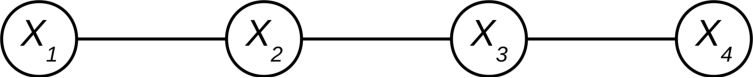
\includegraphics[width=0.4\columnwidth]{./figs/17_2_a.pdf}
      \label{fig:chap_17_2_a}
    \end{figure}
  \end{exerciseSection}
  
  \begin{exerciseSection}
    Same as (a).
  \end{exerciseSection}
  
  \begin{exerciseSection}
    \begin{figure}[htb]
      \centering
      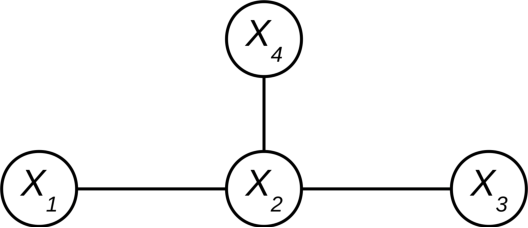
\includegraphics[width=0.3\columnwidth]{./figs/17_2_c.pdf}
      \label{fig:chap_17_2_c}
    \end{figure}
  \end{exerciseSection}
\end{exercise}

\begin{exercise}
  \begin{exerciseSection}
    Since
    \begin{align}
      \left[
        \begin{array}{cc}
          \mathbf{\Theta}_{aa} & \mathbf{\Theta}_{ab} \\
          \mathbf{\Theta}_{ba} & \mathbf{\Theta}_{bb}
        \end{array}
      \right]
      \left[
        \begin{array}{cc}
          \mathbf{\Sigma}_{aa} & \mathbf{\Sigma}_{ab} \\
          \mathbf{\Sigma}_{ba} & \mathbf{\Sigma}_{bb}
        \end{array}
      \right] = \mathbf{I}
    \end{align}
    therefore we have
    \begin{subequations}
      \begin{align}
        \mathbf{\Theta}_{aa}\mathbf{\Sigma}_{aa} +
        \mathbf{\Theta}_{ab}\mathbf{\Sigma}_{ba} = \mathbf{I}
        \label{eq:chap_17_3_a_1}
        \\
        \mathbf{\Theta}_{aa}\mathbf{\Sigma}_{ab} +
        \mathbf{\Theta}_{ab}\mathbf{\Sigma}_{bb} = \mathbf{0}
        \label{eq:chap_17_3_a_2}
      \end{align}
    \end{subequations}
    \eqref{eq:chap_17_3_a_1} -
    \eqref{eq:chap_17_3_a_2}$\mathbf{\Sigma}_{bb}^{-1}\mathbf{\Sigma}_{ba}$, we
    have
    \begin{align}
      \mathbf{\Theta}_{aa}\left(\mathbf{\Sigma}_{aa} -
      \mathbf{\Sigma}_{ab} \mathbf{\Sigma}_{bb}^{-1}\mathbf{\Sigma}_{ba} \right)
      = \mathbf{I}
    \end{align}
    consequently $\mathbf{\Theta}_{aa}^{-1} = \mathbf{\Sigma}_{a, b}$.
  \end{exerciseSection}
  
  \begin{exerciseSection}
    Assume that $\Sigma_{12} = 0$, i.e. $\mathbf{\Sigma}_{aa}$ is diagonal. From
    (a) $\mathbf{\Sigma}_{a, b}$ is also diaonal, which suggests that
    $\mbox{cov}(X_1, X_2|\mbox{rest}) = 0$.
  \end{exerciseSection}
  
  \begin{exerciseSection}
    Since $r_{jk} = \Theta_{jk} / \sqrt{\Theta_{jj} \Theta_{kk}}$, for $j=k$, we
    have $r_{jk} = 1$. For $j\not=k$, denote $X_a = (X_k, X_k)$, then
    \begin{align}
      \left[
        \begin{array}{cc}
          \Theta_{jj} & \Theta_{jk} \\ 
          \Theta_{kj} & \Theta_{kk}
        \end{array}
      \right] = \mathbf{\Theta}_{aa} =
      \left[
        \begin{array}{cc}
          \Sigma_{jj|\mbox{rest}} & \Sigma_{jk|\mbox{rest}} \\ 
          \Sigma_{kj|\mbox{rest}} & \Sigma_{kk|\mbox{rest}}
        \end{array}
      \right]^{-1}
    \end{align}
    therefore
    \begin{subequations}
      \begin{align}
        \Theta_{jj} \Sigma_{jj|\mbox{rest}} + \Theta_{jk}
        \Sigma_{kj|\mbox{rest}} &= 1 \\
        \Theta_{jj} \Sigma_{jk|\mbox{rest}} + \Theta_{jk}
        \Sigma_{kk|\mbox{rest}} &= 0 \\
        \Theta_{kj} \Sigma_{jk|\mbox{rest}} + \Theta_{kk}
        \Sigma_{kk|\mbox{rest}} & = 1
      \end{align}
    \end{subequations}
    consequently, we have
    \begin{subequations}
      \begin{align}
        \Theta_{jj} \Sigma_{jj|\mbox{rest}} & = \Theta_{kk}
        \Sigma_{kk|\mbox{rest}} \\
        \Theta_{jk} \Sigma_{kk|\mbox{rest}} & = \Theta_{jj}
        \Sigma_{jk|\mbox{rest}}
      \end{align}
    \end{subequations}
    As a result, $r_jk = -\Sigma_{jk|\mbox{rest}} /
    \sqrt{\Sigma_{jj|\mbox{rest}} \Sigma_{kk|\mbox{rest}}} =
    -\rho_{jk|\mbox{rest}}$.
  \end{exerciseSection}
\end{exercise}

\begin{exercise}
  Since
  \begin{align}
    f(X_1|X_2, \mbox{rest}) = \frac{f(X_1, X_2| \mbox{rest})}{f(X_2|
    \mbox{rest})} = f(X_1|\mbox{rest})
  \end{align}
  we have
  \begin{align}
    f(X_1, X_2| \mbox{rest}) = f(X_1|\mbox{rest}) f(X_2|\mbox{rest})
  \end{align}
  i.e. $X_1\perp X_2|\mbox{rest}$.
\end{exercise}

\begin{exercise}
  Since there is no missing edges
  \begin{align}
    l_C(\mathbf{\Theta}) = l(\mathbf{\Theta}) = \log|\mathbf{\Theta}| -
    \tr(\mathbf{S\Theta})
  \end{align}
  The gradient equation for maximizing $l_C(\mathbf{\Theta})$ becomes
  $\mathbf{\Theta}^{-1} - \mathbf{S} = 0$, which suggests
  \begin{align}
    \mathbf{S\Theta} = 
    \left[
      \begin{array}{cc}
        \mathbf{S}_{11} & \mathbf{s}_{12} \\
        \mathbf{s}_{12}^T & s_{22}
      \end{array}
    \right]
    \left[
      \begin{array}{cc}
        \mathbf{\Theta}_{11} & \bm{\theta}_{12} \\
         \bm{\theta}_{12}^T & \theta_{22}
      \end{array}
    \right] = 
    \left[
      \begin{array}{cc}
        \mathbf{I} & \mathbf{0} \\
         \mathbf{0}^T & 1
      \end{array}
    \right] 
  \end{align}
  therefore
  \begin{align}
    \mathbf{S}_{11}\bm{\theta}_{12} + \theta_{22}\mathbf{s}_{12} = 0
  \end{align}
  Since $\bm{\beta} = -\bm{\theta}_{12} / \theta_{22}$ as in (17.9), we have
  $\mathbf{S}_{11}\bm{\beta} - \mathbf{s}_{12} = 0$.
\end{exercise}

\begin{exercise}
  Since 
  \begin{align}
    \left[
      \begin{array}{cc}
        \mathbf{W}_{11} & \mathbf{w}_{12} \\
        \mathbf{w}_{12}^T & w_{22}
      \end{array}
    \right]
    \left[
      \begin{array}{cc}
        \mathbf{\Theta}_{11} & \bm{\theta}_{12} \\
         \bm{\theta}_{12}^T & \theta_{22}
      \end{array}
    \right] = 
    \left[
      \begin{array}{cc}
        \mathbf{I} & \mathbf{0} \\
         \mathbf{0}^T & 1
      \end{array}
    \right] 
  \end{align}
  we have
  \begin{subequations}
    \begin{align}
      \mathbf{W}_{11}\bm{\theta}_{12} + \theta_{22}\mathbf{w}_{12} & = 0 \\
      \mathbf{w}_{12}^T\bm{\theta}_{12} + \theta_{22}w_{22} & = 1
    \end{align}
  \end{subequations}
  therefore
  \begin{subequations}
    \begin{align}
      \bm{\theta}_{12} &= -\mathbf{W}_{11}^{-1}\mathbf{w}_{12}\theta_{22} =
      -\hat{\bm{\beta}}\theta_{22} \\
      \theta_{22} &= \frac{1 - \mathbf{w}_{12}^T\bm{\theta}_{12}}{w_{22}}
    \end{align}
  \end{subequations}
  Combining these 2 equations, we have
  \begin{align}
    \theta_{22} = \frac{1}{w_22 -
    \mathbf{w}_{12}^T\mathbf{W}_{11}^{-1}\mathbf{w}_{12}}
  \end{align}
\end{exercise}

\begin{exercise}[(Program)]
\end{exercise}

\begin{exercise}[(Program)]
\end{exercise}

\begin{exercise}
  \begin{exerciseSection}
    \emph{E-step:} The missing data (latent variables), given the current
    estimation $\hat{\bm{\mu}}$, $\hat{\mathbf{\Sigma}}$ and the observed data,
    follow Gaussian distribution as
    \begin{align}
      \mathbf{x}_{i, m_i}\sim\mathcal{N}\left(\hat{\bm{\mu}}_{m_i} +
     \hat{\mathbf{\Sigma}}_{m_i, o_i} \hat{\mathbf{\Sigma}}_{o_i,
      o_i}^{-1} (\mathbf{x}_{i, o_i} - \hat{\bm{\mu}}_{o_i}),
      \hat{\mathbf{\Sigma}}_{m_i, m_i} - \hat{\mathbf{\Sigma}}_{m_i, o_i}
      \hat{\mathbf{\Sigma}}_{o_i, o_i}^{-1} \hat{\mathbf{\Sigma}}_{o_i, m_i}
      \right)
    \end{align}
    (here $\mathbf{x}_{i, m_i}$, $\mathbf{x}_{i, o_i}$ and
    $\hat{\bm{\mu}}_{m_i}$, $\hat{\bm{\mu}}_{o_i})$ are written as column
    vectors.) Therefore, the expectation of the log-likelihood of the data
    over the above conditional distribtion of $\mathbf{x}_{i, m_i}$ is
    \begin{align}
      \mathbb{E}\left[l(\bm{\mu}, \mathbf{\Sigma}; \mathbf{X}_o,
      \mathbf{X}_m)\right] & = C+ N\log|\mathbf{\Sigma}^{-1}| -
      \tr\left(\mathbb{E}\left[(\mathbf{X} - \mathbf{1}\bm{\mu}^T)
      \mathbf{\Theta} (\mathbf{X} - \mathbf{1}\bm{\mu}^T)^T \right] \right)
      \notag
      \\
      &=  C+ N\log|\mathbf{\Sigma}^{-1}|-
      \sum_{i=1}^N
      \sum_{j=1}^p \sum_{k=1}^p\mathbb{E}\left[(x_{ij} - \mu_j)\Theta_{jk}
      (x_{ik} - \mu_k) \right]
    \end{align}
    where $\mathbf{\Theta} = \mathbf{\Sigma}^{-1}$
        
    \emph{M-step: } To maximize the log likelihood, we have
    \begin{align}
      \pdv{\mathbb{E}\left[l(\bm{\mu}, \mathbf{\Sigma}; \mathbf{X}_o,
      \mathbf{X}_m)\right]}{\bm{\mu}} &= \mathbf{1}^T\mathbb{E}[\mathbf{X} -
      \mathbf{1}\bm{\mu}^T]\mathbf{\Theta} = \mathbf{0}
    \end{align}
    thus $\hat{\bm{\mu}} = \mathbb{E}[\mathbf{X}^T\mathbf{1}] / N =
    \hat{\mathbf{X}}^T\mathbf{1} / N$, where $\hat{\mathbf{X}}$ represents the
    $N$-by-$p$ predictor matrix with the missing entries replaced by the imputed
    ones, namely the mean of $\mathbf{x}_{i, m_i}$. Also we have
    \begin{align}
      \pdv{\mathbb{E}\left[l(\bm{\mu}, \mathbf{\Sigma}; \mathbf{X}_o,
      \mathbf{X}_m)\right]}{\mathbf{\Theta}} &= N\mathbf{\Sigma} -
      \mathbb{E} \left[(\mathbf{X} - \mathbf{1}\bm{\mu}^T)^T(\mathbf{X} -
      \mathbf{1}\bm{\mu}^T) \right] = \mathbf{0}
    \end{align}
    therefore, the ML estimation of $\mathbf{\Sigma}$ is
    \begin{align}
      \hat{\mathbf{\Sigma}} = \frac{1}{N} \mathbb{E} \left[(\mathbf{X} -
      \mathbf{1}\hat{\bm{\mu}}^T)^T(\mathbf{X} - \mathbf{1}\hat{\bm{\mu}}^T)
      \right]
    \end{align}
    Denote $E_{ijk} = \mathbb{E}\left[(x_{ij} - \hat{\mu}_j)(x_{ik} -
    \hat{\mu}_k) \right]$, since
    \begin{align}
      E_{ijk} &= (\mathbb{E}[x_{ij}] - \hat{\mu}_j)(\mathbb{E}[x_{ik}] -
      \hat{\mu}_k) + \mbox{cov}(x_{ij}x_{ik})
    \end{align}
    in which 
    \begin{align}
      \mathbb{E}[x_{ij}] = \hat{x}_{ij},\;\mathbb{E}[x_{ik}] = \hat{x}_{ik}
    \end{align}
    whether $j,k\in m_i$ or not, and
    \begin{align}
      \mbox{cov}(x_{ij}x_{ik}) = \left\{
        \begin{array}{ll}
          0 & \mbox{if } j\in o_i \mbox{ or } k\in o_i \\
          \hat{\Sigma}_{jk} & \mbox{otherwise}
        \end{array}
      \right.
    \end{align}
    therefore (17.44) is proved, in which the correction term $c_{i, jj'}$
    corresponds to the the non-zero covariance $\mbox{cov}(x_{ij}x_{ij'})$ when
    both $j$ and $j'$ are imputed for $x_i$.
  \end{exerciseSection}
  
  \begin{exerciseSection}
    (Program)
  \end{exerciseSection}
  
  \begin{exerciseSection}
    (Program)
  \end{exerciseSection}
\end{exercise}

\begin{exercise}
  An absence of the constant node $X_0 \equiv 1$ ill lead to the following
  ambiguity
  \begin{align}
    p(X_1=0, X_2=0) = p(X_1=1, X_2=0) = p(X_1=0, X_2=1)
  \end{align}
  only by including $X_0 \equiv 1$ the 4 possible values can be uniquely
  defined. \begin{figure}[htb]
      \centering
      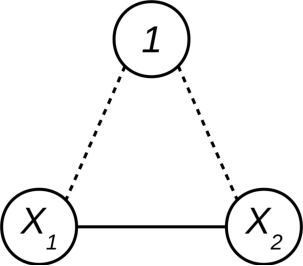
\includegraphics[width=0.15\columnwidth]{./figs/17_10.pdf}
      \label{fig:chap_17_10}
    \end{figure}
\end{exercise}

\begin{exercise}
  \begin{align}
    p(X_j=1|X_{\mbox{rest}} = x_{\mbox{rest}}, \mathbf{\Theta}) &=
    \frac{p(X_j=1,X_{\mbox{rest}} = x_{\mbox{rest}} |
    \mathbf{\Theta})}{p(X_{\mbox{rest}} = x_{\mbox{rest}} | \mathbf{\Theta})}
    \notag \\
    &= \frac{p(X_j=1,X_{\mbox{rest}} = x_{\mbox{rest}} |
    \mathbf{\Theta})} {p(X_j=1, X_{\mbox{rest}} = x_{\mbox{rest}} |
    \mathbf{\Theta}) + p(X_j=0, X_{\mbox{rest}} = x_{\mbox{rest}} |
    \mathbf{\Theta})} \notag \\
    &= \frac{C\exp\left(\sum_{k:(j,k)\in
    E}\theta_{jk}x_k\right)}{C\exp\left(\sum_{k:(j,k)\in E}\theta_{jk}x_k\right)
    + C} \notag \\
    &= \frac{1} 
    {1 + \exp\left(-\sum_{k:(j,k)\in E}\theta_{jk}x_k\right)}
  \end{align}
  where $C$ is a constant given the value of the rest nodes in the graph. Now
  this probability has the logistic form as (17.30) (considering a
  constant node $X_0=1$).
\end{exercise}

\begin{exercise}
  ???
\end{exercise} % Chapter 17
\chapter{High-Dimensional Problems}
\label{ch:18}

\begin{exercise}
  ???
\end{exercise}

\begin{exercise}
  To minimize the lasso-style objective function (denoted as $L$), we have
  \begin{subequations}
    \begin{align}
      \pdv{L}{\mu_j} & = \sum_{k=1}^K\sum_{i\in C_k}-\frac{x_{ij}- \mu_j -
      \mu_{jk}} {s_j^2} = 0 \\
      \pdv{L}{\mu_{jk}} & = \sum_{i\in C_k} -\frac{x_{ij}- \mu_j - \mu_{jk}}
      {s_j^2} + \lambda\sqrt{N_k}\frac{\mbox{sign}(\mu_{jk})}{s_j} = 0
    \end{align}
  \end{subequations}
  therefore
  \begin{subequations}
    \begin{align}
      \mu_{jk} & = \bar{x}_{jk} - \mu_j -
      \frac{\lambda s_j \mbox{sign}(\mu_{jk})}{\sqrt{N_k}} \\
      \mu_j &= \bar{x}_j - \frac{1}{N}\sum_{k=1}^KN_k\mu_{jk}
    \end{align}
  \end{subequations}
  wher $\bar{x}_{jk} = \sum_{i\in C_k}x_{ij} / N_k$ and $\bar{x}_j =
  \sum_{i=1}^Nx_{ij} / N$. (Here we note that the condition
  $\sum_{k=1}^K\mu_{jk}$ should have been $\sum_{k=1}^KN_k\mu_{jk} = 0$.)
  Consequently
  \begin{align}
    \mu_{jk} = \bar{x}_{jk}- \bar{x}_j - \frac{\lambda s_j
    \mbox{sign}(\mu_{jk})}{\sqrt{N_k}},
  \end{align}
  therefore
  \begin{align}
    d_{kj}' &= \frac{\sqrt{N_k}\mu_{jk}}{s_j} \notag \\
    &= \frac{\bar{x}_{jk}- \bar{x}_j}{m_k(s_j + s_0)} -
    \lambda\mbox{sign}(d_{kj}') \notag \\
    &= d_{kj} - \lambda\mbox{sign}(d_{kj}')
  \end{align}
  where $s_0 = 0$ and $m_k = 1 /\sqrt{N_k}$. As a result, we have $d_{kj}' =
  \mbox{sign}(d_{kj})(|d_{kj} - \Delta|)_+$, where $\Delta = \lambda$.
\end{exercise}

\begin{exercise}
  The penalized log-likelihood objective function in (18.11) is explicitly
  written as
  \begin{align}
    l_P(\bm{\beta}_0, \mathbf{B}; \mathbf{X}, \mathbf{g}) &= \sum_{i=1}^N 
    \left[\beta_{k_i0} + \mathbf{x}_i^T\bm{\beta}_{k_i} - \log \sum_{l=1}^K 
    \exp(\beta_{l0} + \mathbf{x}_i^T\bm{\beta}_l) \right] - \frac{\lambda}{2}
    \sum_{k=1}^K\|\bm{\beta}_k\|^2
  \end{align}
  The necessary condition to maximize the penalized log-likelihood is
  \begin{align}
    \pdv{l_P(\bm{\beta}_0, \mathbf{B}; \mathbf{X}, \mathbf{g})}{\bm{\beta}_k} &=
    \sum_{i:g_i=k}\mathbf{x}_i^T - \sum_{i=1}^N\mbox{Pr}(k|\mathbf{x}_i)
    \mathbf{x}_i^T - \lambda\bm{\beta}_k^T = \mathbf{0}
  \end{align}
  for $k=1,\ldots,K$. Consequently,
  \begin{align}
    \sum_{k=1}^K  \pdv{l_P(\bm{\beta}_0, \mathbf{B}; \mathbf{X},
    \mathbf{g})}{\bm{\beta}_k} &= \mathbf{0} \notag \\
    &= \sum_{i=1}^N\mathbf{x}_i^T - \sum_{i=1}^N \left(\sum_{k=1}^K
    \mbox{Pr}(k|\mathbf{x}_i)\right)\mathbf{x}_i^T - \lambda
    \sum_{k=1}^K\bm{\beta}_k^T \notag \\
    &=  - \lambda \sum_{k=1}^K\bm{\beta}_k^T
  \end{align}
  therefore $\sum_{k=1}^K\beta_{kj} = 0$, $j=1,\ldots,p$. $\beta_{k0}$ should
  all be set to 0.
\end{exercise}

\begin{exercise}
  \begin{align}
    \hat{\bm{\beta}} &= (\mathbf{X}^T\mathbf{X} + \lambda \mathbf{I})^{-1}
    \mathbf{X}^T \mathbf{y} \notag \\
    &= (\mathbf{VR}^T\mathbf{RV}^T + \lambda \mathbf{I})^{-1}\mathbf{VR}^T
    \mathbf{y} \notag \\
    &= \left[\lambda^{-1}\mathbf{I} - \lambda^{-1}\mathbf{V}
    \left((\mathbf{R}^T\mathbf{R})^{-1} + \lambda^{-1}\mathbf{I}
    \right)^{-1}\mathbf{V}^T \lambda^{-1}\right] \mathbf{VR}^T\mathbf{y}
    \notag\\
    & = \lambda^{-1}\mathbf{V} \left[\mathbf{I} - \lambda^{-1}
    \left((\mathbf{R}^T\mathbf{R})^{-1} + \lambda^{-1}\mathbf{I} \right)^{-1}
    \right]\mathbf{R}^T\mathbf{y} \notag\\
    &= \lambda^{-1}\mathbf{V} \left[\mathbf{I} - \lambda^{-1}
    \left(\lambda\mathbf{I} - \lambda^2(\mathbf{R}^T\mathbf{R} +
    \lambda\mathbf{I})^{-1} \right) \right]\mathbf{R}^T\mathbf{y} \notag \\
    &= \mathbf{V} (\mathbf{R}^T\mathbf{R} +
    \lambda\mathbf{I})^{-1} \mathbf{R}^T\mathbf{y}
  \end{align}
  Through this proof we have made use of the Woodbury matrix identity twice.
  (What has it to do with the hint?)
\end{exercise}

\begin{exercise}
  $\forall\bm{\beta}, \beta_0$, let $\theta_0 = \beta_0$ and decompose
  $\bm{\beta}$ as $\bm{\beta} = \mathbf{V}\bm{\theta} +
  \mathbf{V}_{\perp}\bm{\theta}_{\perp}$, where $\mathbf{V}_{\perp}$
  is a set of orthonormal vectors representing the complementary space of 
  $\mathbf{V}$.
  Consequently
  \begin{subequations}
    \begin{align}
      \mathbf{X}\bm{\beta} + \beta_0\mathbf{1} & = \mathbf{R}\bm{\theta} +
      \theta_0\mathbf{1} \\
      \bm{\beta}^T\bm{\beta} = \bm{\theta}^T\bm{\theta} & +
      \bm{\theta}_{\perp}^T\bm{\theta}_{\perp} \geq \bm{\theta}^T\bm{\theta}
    \end{align}
  \end{subequations}
  This suggests that a solution to (18.16) must have $\hat{\bm{\theta}}_{\perp}
  = \mathbf{0}$. Consequently, the solution to (18.16) can be constructed from
  the solution to (18.17) by $\hat{\bm{\beta}} = \mathbf{V}\hat{\bm{\theta}}$,
  $\hat{\beta}_0 = \hat{\theta}_0$.
\end{exercise}

\begin{exercise}
  (Not Section 4.14 but equation (4.14).) Write the regularized discriminant
  analysis (RDA) into the ASR form in (12.57):
  \begin{align}
    ASR = \frac{1}{N}\sum_{l=1}^L \left[\sum_{i=1}^N \left(\theta_l(g_i) -
    \beta_{l0} - \mathbf{x}_i^T\mathbf{\bm{\beta}}_l \right)^2 +
    \frac{1-\gamma}{\gamma} \hat{\sigma}^2\bm{\beta}_l^T\bm{\beta}_l \right]
  \end{align}
  which is now in the form as in Sec.18.3.5. By defining $\beta_{l0} = u_{l0}$,
  $\bm{\beta}_l = \mathbf{V}\mathbf{u}_l$, we can solve a smaller problem for
  $\hat{u}_{l0}, \hat{\mathbf{u}}_l$, $l=1,\ldots,L$ then map them back to get
  $\hat{\beta}_{l0}, \hat{\bm{\beta}}_l$.
\end{exercise}

\begin{exercise}
  \begin{exerciseSection}
    As $\mathbf{y} = \mathbf{X}\bm{\beta}$, we have
    $\mathbf{R}^{-1}\mathbf{y} = \mathbf{V}^T\bm{\beta}$. Since $\mathbf{V}^T$
    has rank $N$, this equation must have at least 1 solution denoted as
    $\bm{\beta}_0$. Consequently, 
    \begin{align}
      \bm{\beta} = \bm{\beta}_0 + \mathbf{V}_{\perp}\bm{\beta}_{\perp}
    \end{align}
    where $\mathbf{V}_{\perp}$ (rank $N - p$) represent the complementary space
    of $\mathbf{V}$, is a solution for arbitrary $\bm{\beta}_{\perp}$.
  \end{exerciseSection}
  
  \begin{exerciseSection}
    Same as Ex. (18.4).
  \end{exerciseSection}

  \begin{exerciseSection}
    \begin{align}
      \mathbf{X}\hat{\bm{\beta}}_0 =
      \mathbf{UDV}^T\mathbf{VD}^{-1}\mathbf{U}^T\mathbf{y} = \mathbf{y}
    \end{align}
    thus there is zero residual. Denote a solution as $\bm{\beta} =
    \mathbf{V}\bm{\theta} + \mathbf{V}_{\perp}\bm{\theta}_{\perp}$. Since 
    $\mathbf{y} = \mathbf{X}\bm{\beta} = \mathbf{R}\bm{\theta}$, we have
    $\bm{\theta} = \mathbf{R}^{-1}\mathbf{y}$, therefore $\bm{\beta}$ can be
    rewritten as
    \begin{align}
      \beta = \mathbf{VR}^{-1}\mathbf{y} + \mathbf{V}_{\perp}\bm{\theta}_{\perp}
    \end{align}
    Since $\|\beta \|^2 = \|\mathbf{R}^{-1}\mathbf{y}\|^2 +
    \|\bm{\theta}_{\perp}\|^2 \leq \|\mathbf{R}^{-1}\mathbf{y}\|^2$, in which
    equality holds iff $\beta = \mathbf{VR}^{-1}\mathbf{y}$. As a result, it
    is unique with the smallest Euclidean norm.
  \end{exerciseSection}
\end{exercise}

\begin{exercise}
  \begin{exerciseSection}
    Decompose $\mathbf{X} = \mathbf{RV}^T$. Then $\mathbf{X}\bm{\beta}$ projects
    to $\pm(1-\alpha)$ for $\bm{\beta} = \mathbf{VR}^{-1}\mathbf{y} + \mathbf{V}_{\perp}\bm{\beta}_{\perp}$
  \end{exerciseSection}
  
  \begin{exerciseSection}
    Since
    \begin{align}
      \frac{\mathbf{x}_i^T\hat{\bm{\beta}}} {\|\hat{\bm{\beta}}\|} =
      \frac{\pm(1-\alpha)}{\hat{\bm{\beta}}}
    \end{align}
    therefore the distance is $2/\hat{\bm{\beta}}$.
  \end{exerciseSection}
  
  \begin{exerciseSection}
    Same as Ex 18.7. Largest distance achieved by $\hat{\bm{\beta}}_0$ which has
    the smallest Euclidean norm.
  \end{exerciseSection}
\end{exercise}

\begin{exercise}
  Apparently optimal separating hyperplane makes the widest margin by its
  definition. Specifically, (4.48) when $p\gg N$ must have a solution
  $\tilde{\bm{\beta}}$, which means $\forall i, j$ such that $y_i = 1$,
  $y_j=-1$, we have
  \begin{align}
    \mathbf{x}_i^T\tilde{\bm{\beta}} + \tilde{\beta}_0 \geq 1,\;
    \mathbf{x}_j^T\tilde{\bm{\beta}} + \tilde{\beta}_0 \leq 1
  \end{align}
  Consequently the margin is at least $2/\|\tilde{\bm{\beta}}\|$. Also we must
  have $\|\tilde{\bm{\beta}}\| \leq \|\hat{\bm{\beta}}_0\|$, since the later is
  also valid for the constraints in (4.48). As a result, optimal separating
  hyperplane separates data by a wider margin then does the data piling
  direction.
\end{exercise}

\begin{exercise}
  Decompose $\mathbf{X}$ into $\mathbf{X}=\mathbf{RV}^T$. Then we can project
  $\bar{\mathbf{x}}_1$ and $\bar{\mathbf{x}}_{-1}$ onto $\mathbf{V}$ as
  \begin{align}
    \bar{\mathbf{r}}_1 = \mathbf{V}^T\bar{\mathbf{x}}_1, &\;
    \bar{\mathbf{r}}_{-1} = \mathbf{V}^T\bar{\mathbf{x}}_{-1} \\
    \bar{\mathbf{x}}_1 = \mathbf{V}\bar{\mathbf{r}}_1, &\; 
    \bar{\mathbf{x}}_{-1} = \mathbf{V}\bar{\mathbf{r}}_{-1}
  \end{align}
  and the within-class variance matrix for $\mathbf{R}$ satisfies $\mathbf{W} =
  \mathbf{V}\mathbf{W}_R\mathbf{V}^T$. For any $\mathbf{x}$, we decompose it
  into $\mathbf{x} = \mathbf{Vr} + \mathbf{V}_{\perp}\mathbf{r}_{\perp}$. Then
  the discrimant function becomes
  \begin{align}
    & \mathbf{x}^T(\mathbf{W} + \lambda\mathbf{I})^{-1}(\bar{\mathbf{x}}_1 -
    \bar{\mathbf{x}}_{-1}) \notag \\
    = & (\mathbf{r}^T\mathbf{V}^T + \mathbf{r}_{\perp}^T\mathbf{V}_{\perp}^T)
    (\mathbf{V}\mathbf{W}_R\mathbf{V}^T +
    \lambda\mathbf{I})^{-1}\mathbf{V}(\bar{\mathbf{r}}_1 -
    \bar{\mathbf{r}}_{-1}) \notag \\
    = & (\mathbf{r}^T\mathbf{V}^T + \mathbf{r}_{\perp}^T\mathbf{V}_{\perp}^T)
    \mathbf{V}(\mathbf{W}_R + \lambda\mathbf{I})^{-1}(\bar{\mathbf{r}}_1 -
    \bar{\mathbf{r}}_{-1})\notag \\
    = & \mathbf{r}^T(\mathbf{W}_R + \lambda\mathbf{I})^{-1}(\bar{\mathbf{r}}_1 -
    \bar{\mathbf{r}}_{-1})
  \end{align}
  where the proof is similar to Ex. 18.4. Consequently, the discriminant
  function can be redefined on $\mathbf{r}$:
  \begin{align}
    \delta_0(\mathbf{r}) = \lim_{\lambda\rightarrow 0}\delta(\mathbf{r}) =
    \mathbf{r}^T \mathbf{W}_R^{-1}(\bar{\mathbf{r}}_1 -
    \bar{\mathbf{r}}_{-1})
  \end{align}
  
  On the other hand, for the solution $\hat{\bm{\beta}}$ to the linear response
  regression to binary response $\pm1$, we have $\mathbf{x}^{T}\hat{\bm{\beta}} =
  \mathbf{r}^{T}\mathbf{R}^{-1}\mathbf{y}$.
  According to Ex. 4.2 we have $\mathbf{R}^{-1}\mathbf{y} \propto
  \mathbf{W}_R^{-1}(\bar{\mathbf{r}}_1 - \bar{\mathbf{r}}_{-1})$ (Assuming
  $N_1=N_2$). Consequently $\delta_0(\mathbf{r})$ is equivalent to the
  projection onto the maximal data piling direction up to scaling.
\end{exercise}

\begin{exercise}
  The optimal solution is characterized by (4.21)
  \begin{align}
    \pdv{l(\bm{\beta})}{\bm{\beta}} = \sum_{i=1}^N\mathbf{x}_i^T 
    \left(y_i - \frac{\exp(\alpha + \mathbf{x}_i^T\bm{\beta})}{1 + \exp(\alpha +
    \mathbf{x}_i^T\bm{\beta})} \right) = \mathbf{0}
  \end{align}
  If $\bm{\beta}_0$ is a solution, then $\bm{\beta}_0 + \Delta\bm{\beta}$ where
  $\mathbf{X}\Delta\bm{\beta} = \mathbf{0}$ is also a solution. Since $p\gg N$,
  there are intinitely many $\Delta\bm{\beta}$. Consequently, $\bm{\beta}$ is
  undefined.
\end{exercise}

\begin{exercise}
  $\mathbf{X} = \mathbf{RV}^T$ implies that $\mathbf{X}_B =
  \mathbf{R}_B\mathbf{V}^T$, where $\mathbf{R}_B$ corresponds to the same rows
  in $\mathbf{R}$ as does the CV samples $\mathbf{X}_B$ to $\mathbf{X}$.
  Consequetnly, we need to reduce $\mathbf{X}$ to $\mathbf{R}$ only once, and CV
  fitting can be done on subsets of rows of $\mathbf{R}$.
\end{exercise}

\begin{exercise}
  Denot the logit function as $\mbox{logit}(\mathbf{x}) = a_0 +
  \mathbf{x}^T\mathbf{a}$, then the ridged logistic regression is in the form of
  \begin{align}
    \min_{a_0, \mathbf{a}} \sum_{i=1}^N y_i\log\frac{\exp(a_0 +
    \mathbf{x}_i^T\mathbf{a})}{1 + \exp(a_0 + \mathbf{x}_i^T\mathbf{a})}
    + (1 - y_i)\log\frac{1}{1 + \exp(a_0 + \mathbf{x}_i^T\mathbf{a})} 
    + \lambda\|\mathbf{a}\|^2
  \end{align}
  Similar to Ex 18.7, denote $\beta_0 = a_0$, $\mathbf{a} =
  \mathbf{V}\bm{\beta}$, this problem is equivalent to the ridged logistic
  regression in $\mathbf{R}$ instead of $\mathbf{X}$ where $\mathbf{X} =
  \mathbf{RV}^T$:
  \begin{align}
    \min_{\beta_0, \bm{\beta}} \sum_{i=1}^N y_i\log\frac{\exp(\beta_0 +
    \mathbf{r}_i^T\bm{\beta})}{1 + \exp(\beta_0 + \mathbf{r}_i^T\bm{\beta})}
    + (1 - y_i)\log\frac{1}{1 + \exp(\beta_0 + \mathbf{r}_i^T\bm{\beta})} 
    + \lambda\|\bm{\beta}\|^2
  \end{align}
  Then the predictions are given by
  \begin{align}
    \hat{f}_0 & = \hat{a}_0 + \mathbf{x}_0^T\hat{\mathbf{a}} \notag \\
    &= \hat{\beta}_0 + \mathbf{x}_0^T\mathbf{V}\hat{\bm{\beta}} \notag \\
    &= \hat{\beta}_0 + \mathbf{x}_0^T\mathbf{VDU}^T\mathbf{UD}^{-1}
    \hat{\bm{\beta}} \notag \\
    &= \hat{\beta}_0 + \mathbf{k}_0^T \mathbf{UD}^{-1}\hat{\bm{\beta}}
  \end{align}
  therefore $\hat{\alpha} = \mathbf{UD}^{-1}\hat{\bm{\beta}}$.
  
  With the logit function in kernel space
  $\mbox{logit}(\mathbf{x}) = h(\mathbf{x}), h\in\mathcal{H}_K$, the kernel
  ridged logistic regression problem is
  \begin{align}
    \min_{h\in\mathcal{H}_K} = \sum_{i=1}^N y_i\log\frac{\exp(h(\mathbf{x}_i))}
    {1 + \exp(h(\mathbf{x}_i))} + (1 - y_i)\log\frac{1}{1 +
    \exp(h(\mathbf{x}_i))} + \lambda\|h\|_{\mathcal{H}_K}^2
  \end{align}
  According to (5.48), the solution must be in the form of
  \begin{align}
    h(\mathbf{x}) = \sum_{i=1}^N\beta_iK(\mathbf{x}, \mathbf{x}_i)
  \end{align}
  therefore the ridged regression can be rewritten as
  \begin{align}
    \min_{\bm{\beta}} \sum_{i=1}^N y_i\log\frac{\exp(\mathbf{k}_i^T\bm{\beta})}
    {1 + \exp(\mathbf{k}_i^T\bm{\beta})} + (1 - y_i)\log\frac{1}{1 +
    \exp(\mathbf{k}_i^T\bm{\beta})} + \lambda\bm{\beta}^T\mathbf{K}\bm{\beta}
  \end{align}
  where $\mathbf{k}_i$ is the $i$-th column of $\mathbf{K}$. Denote $\mathbf{b}
  = \mathbf{DU}^T\bm{\beta}$, then the ridged regression is equivalent to
  \begin{align}
    \min_{\mathbf{b}} \sum_{i=1}^N y_i\log\frac{\exp(\mathbf{r}_i^T\mathbf{b})}
    {1 + \exp(\mathbf{r}_i^T\mathbf{b})} + (1 - y_i)\log\frac{1}{1 +
    \exp(\mathbf{r}_i^T\mathbf{b})} + \lambda\|\mathbf{b}\|^2
  \end{align}
  Assuming the optimal solution $\mathbf{b}$, then the prediction is
  \begin{align}
    h(\mathbf{x}_0) = \mathbf{k}_0^T\hat{\beta} = \mathbf{k}_0^T
    \mathbf{UD}^{-1}\mathbf{b}
  \end{align}
  where $\mathbf{k}_0 = [K(\mathbf{x}_0, \mathbf{x}_1),\ldots, K(\mathbf{x}_0,
  \mathbf{x}_N)]^T$.
\end{exercise}

\begin{exercise}
  \begin{exerciseSection}
    \begin{align}
      f_+(x_0) & \approx \frac{\mbox{Total number in class +1 in this
      region}}{(\mbox{Total number in class +1})(\mbox{Volumn of this region})}
      \notag \\
      & = \frac{1}{N_+d_+(x_0)^p}
    \end{align}
    Therefore the discriminant function
    \begin{align}
      \delta(x_0) = \log\frac{p_+(x_0)}{p_-(x_0)} =
      \log\frac{\pi_+f_+(x_0)}{\pi_-f_-(x_0)}
    \end{align}
    If we estimate the prior distribution as $\pi_+ = N_+ / N$, $\pi_- = N_- /
    N$, then 
    \begin{align}
      \delta(x_0) = p\log\frac{d_-(x_0)}{d_+(x_0)}
    \end{align}
  \end{exerciseSection}
  
  \begin{exerciseSection}
    If $\pi_+$, $\pi_-$ is given, then 
    \begin{align}
      \delta(x_0) = \log\frac{\pi_+}{\pi_-} + \log\frac{N_-}{N_+} + 
      p\log\frac{d_-(x_0)}{d_+(x_0)}
    \end{align}
  \end{exerciseSection}
  
  \begin{exerciseSection}
    Simply redefine $d_+(x_0)$ as the smallest distance within which there are
    $k$ samples in class +1, and $d_-(x_0)$ as the smallest distance within
    which there are $k$ samples in class -1. The results are the same as (a),
    (b).
  \end{exerciseSection}
\end{exercise}

\begin{exercise}
  First we show that the $m$-th component $\mathbf{z}_m$ can be written as
  $z_{im} = \sum_{j=1}^N\alpha_{jm}K(\mathbf{x}_i, \mathbf{x}_j)$ up to
  centering, where $\alpha_{jm} = u_{jm}/d_m$. Since $z_{im}$ is the entry in
  the $i$-th row, $m$-th column of $\mathbf{Z}^T$, where
  \begin{align}
    \mathbf{Z}^T = \mathbf{DU}^T = \mathbf{D}^{-1}\mathbf{U}^T(\mathbf{I} -
    \mathbf{M})\mathbf{K}(\mathbf{I} - \mathbf{M})
  \end{align}
  Therefore $z_{im}$ equals to the product of the $i$-th row of
  $\mathbf{D}^{-1}\mathbf{U}^T$ and the $m$-th column of $(\mathbf{I} -
  \mathbf{M})\mathbf{K}(\mathbf{I} - \mathbf{M})$. Note that the $j$-th element
  of the former is $u_{jm}/d_m$ and the $j$-th element of the latter is
  $\langle h(\mathbf{x}_i) - \bar{h}, h(\mathbf{x}_j) - \bar{h})\rangle$ where
  $\bar{h} = \sum_{j=1}^N h(\mathbf{x}_j) / N$.
  
  Denote the centered projection of $\mathbf{x}_0$ onto the principle component
  direction as $\mathbf{z}_0$, then its $m$-th element is
  \begin{align}
    z_{0m} & = \left\langle h(\mathbf{x}_0) - \bar{h},
    \sum_{j=1}^N\frac{u_{jm}}{d_m} (h(\mathbf{x}_j) - \bar{h})\right\rangle
    \notag \\
    & = \sum_{j=1}^N \frac{u_{jm}}{d_m}\left[\langle h(\mathbf{x}_0),
    h(\mathbf{x}_j)\rangle - \langle h(\mathbf{x}_0), \bar{h} \rangle - \langle
    \bar{h}, h(\mathbf{x}_j) \rangle + \langle \bar{h}, \bar{h} \rangle \right]
    \notag \\
    & = \sum_{j=1}^N \frac{u_{jm}}{d_m} \left[k_{0j} - (\mathbf{Mk}_0)_j -
    (\mathbf{K1})_j / N + \mathbf{1}^T\mathbf{K1} \right]
  \end{align}
  Again $u_{jm}/d_m$ is the $m$-th row, $j$-th column of
  $\mathbf{D}^{-1}\mathbf{U}^T$, and the term in the squared bracket equals to
  the $j$-th element of $(\mathbf{I} - \mathbf{M})[\mathbf{k}_0 -
  \mathbf{K1}/N]$. Consequently,
  \begin{align}
    \mathbf{z}_0 = \mathbf{D}^{-1}\mathbf{U}^T (\mathbf{I} -
    \mathbf{M})[\mathbf{k}_0 - \mathbf{K1}/N]
  \end{align}
\end{exercise}

\begin{exercise}
  \begin{exerciseSection}
    \begin{align}
      \mbox{Pr}(A) = \mbox{Pr}(\cup_{j=1}^MA_j) \leq \sum_{j=1}^M \mbox{Pr}(A_j)
      = \alpha
    \end{align}
  \end{exerciseSection}
  
  \begin{exerciseSection}
    When $\alpha/M$ is small, the first-order approximation
    \begin{align}
      1 - (1 - \alpha/M)^M \approx \alpha
    \end{align}
  \end{exerciseSection}
\end{exercise}

\begin{exercise}
  \begin{exerciseSection}
    Since $p_{(1)} \leq \ldots \leq p_{(M)}$, $|t_1|\geq\ldots\geq|t_M|$, we
    have $|T|_{(L)} = |t_L|$. By definition in (18.41),
    \begin{align}
      p_0 = p_{(L)} = \frac{1}{MK}\sum_{j=1}^M \sum_{k=1}^K I(|t_{j}^k| >
      |t_L|)
    \end{align}
    thus there are at most $p_0$ of $|t_{j}^k| > |t_L| = |T|_{(L)}$. For the
    plug-in estimation, we have
    \begin{align}
      R_{\mbox{obs}} & = \sum_{j=1}^M I(|t_j| > |t_L|) = L \\
      \widehat{\mbox{E}(V)} & = M\cdot \frac{1}{MK}\sum_{j=1}^M \sum_{k=1}^K
      I(|t_{j}^k| > |t_L|) \leq p_0M
    \end{align}
    therefore $\widehat{\mbox{FDR}}\leq p_0M/L = \alpha$.
  \end{exerciseSection}
  
  \begin{exerciseSection}
    According to (18.44)
    \begin{align}
      p_{(L+1)} & > \alpha \frac{L+1}{M} \notag \\
      & = \frac{1}{MK}\sum_{j=1}^M \sum_{k=1}^K I(|t_{j}^k| > |t_{L+1}|) \notag
      \\
      &= \frac{\widehat{\mbox{E}(V)}}{M}
    \end{align}
    Also we have
    \begin{align}
      R_{\mbox{obs}} & = \sum_{j=1}^M I(|t_j| > |t_{L+1}|) = L + 1
    \end{align}
    therefore $\widehat{\mbox{FDR}} =  \widehat{\mbox{E}(V)} / R_{\mbox{obs}} >
    \alpha$.
  \end{exerciseSection}
\end{exercise}

\begin{exercise}
  \begin{align}
    \mbox{pFDR}(\Gamma) &= \frac{\mbox{Pr}(\mbox{$j$-th null hypothesis
    is true and the null hypothesis is rejected})} {\mbox{Pr}(\mbox{$j$-th null
    hypothesis is rejected})} \notag \\
    & = \frac{\mbox{Pr}(Z_j=0,t_j\in\Gamma)}{\mbox{Pr}(t_j\in\Gamma)} \notag\\
    & = \frac{\mbox{Pr}(Z_j=0)\mbox{Pr}(t_j\in\Gamma|Z_j=0)}
    {\mbox{Pr}(Z_j=0)\mbox{Pr}(t_j\in\Gamma|Z_j=0) +
    \mbox{Pr}(Z_j=1)\mbox{Pr}(t_j\in\Gamma|Z_j=1)} \notag \\
    & = \frac{\pi_0 \{\mbox{Type I error of $\Gamma$}\}} {\pi_0 \{\mbox{Type I
    error of $\Gamma$}\} + \pi_1 \{\mbox{Power of $\Gamma$}\}}
  \end{align}
\end{exercise}

\begin{exercise}[(Program)]
\end{exercise}

\begin{exercise}
  \begin{align}
    \mbox{pFDR} & = \mbox{E}\left[\frac{V}{R}|R>0\right] \notag \\
    & = \sum_{k=1}^M \mbox{E}\left[\frac{V}{R}|R=k\right]\mbox{Pr}(R=k|k=0)
  \end{align}
  Since $V$ is binomial distributed from $0$ to $k$ given $k$, the expectation
  of $V$ given $k$ is
  \begin{align}
    \mbox{E}_k[V] = k\mbox{Pr}(H=0|T\in \Gamma)
  \end{align}
  therefore
  \begin{align}
    \mbox{pFDR} & = \sum_{k=1}^M \mbox{Pr}(H=0|T\in \Gamma) \mbox{Pr}(R=k|k=0)
    \notag \\
    &= \mbox{Pr}(H=0|T\in \Gamma)
  \end{align}
\end{exercise} % Chapter 18

\appendix
%\input{./chapters/refs.tex}
\bibliographystyle{apalike}
\bibliography{refs}

\end{document}
